%*******************************************************************
% Chapter 6: Result Analysis
%*******************************************************************

\section{Dense Smoke and Fire Object Detection Benchmark}
\label{sec:object_detection}

To establish dense object detection baselines for UAV disaster monitoring, seven modern detection architectures were evaluated on the \textbf{D-Fire smoke and fire object detection benchmark}~\cite{dfire2022} (21{,}527 images containing bounding box annotations for diffuse smoke plumes and localized flame fronts). Table~\ref{tab:dfire_results} presents the comparative evaluation under standardized COCO evaluation protocols ($mAP_{50}$ and $mAP_{50:95}$).

\begin{table}[H]
\centering
\caption{Dense Smoke and Fire Object Detection Benchmark on D-Fire ($n=21{,}527$ images, 512/640px input). Models are evaluated on localized smoke and flame bounding box detection. Time is the wall-clock duration of each saved training run up to its stopping point; because per-epoch learning curves are not compared, differences in time indicate training cost, not convergence rate.}
\label{tab:dfire_results}
\resizebox{\textwidth}{!}{%
\begin{tabular}{@{}llccccccc@{}}
\toprule
\textbf{Model / Experiment} & \textbf{Architecture} & \textbf{Time (h)} & \textbf{Prec.} & \textbf{Rec.} & \textbf{mAP$_{50}$} & \textbf{mAP$_{50{:}95}$} & \textbf{AP$^{smoke}_{50}$} & \textbf{AP$^{fire}_{50}$} \\
\midrule
YOLO26s (CLAHE) & YOLO26s~\cite{sapkota2025yolo26} & 42.6 & \textbf{0.769} & \textbf{0.701} & \textbf{0.7710} & \textbf{0.4480} & \textbf{0.8485} & \textbf{0.6936} \\
\textbf{RT-DETRv2-R18} & RT-DETRv2-R18~\cite{lv2024rtdetrv2} & 7.85 & 0.742 & 0.678 & \textbf{0.7380} & 0.4215 & 0.8120 & 0.6640 \\
YOLO26n (CLAHE, fine-tune) & YOLO26n~\cite{sapkota2025yolo26} & 4.28 & 0.736 & 0.666 & 0.7258 & 0.4088 & 0.7964 & 0.6551 \\
\textbf{YOLO11n Baseline} & YOLO11n~\cite{ultralytics2024yolo11} & 4.60 & 0.728 & 0.659 & \textbf{0.7225} & 0.4052 & 0.7910 & 0.6540 \\
YOLO26n (baseline) & YOLO26n~\cite{sapkota2025yolo26} & 4.45 & 0.712 & 0.647 & 0.7147 & 0.4005 & 0.7833 & 0.6460 \\
\textbf{Hazard-YOLO26n (HPG)} & \textbf{YOLO26n + HPG} & \textbf{1.96} & 0.715 & 0.636 & \textbf{0.7053} & 0.3989 & 0.7812 & 0.6294 \\
YOLOv10n (baseline) & YOLOv10n~\cite{wang2024yolov10} & 5.07 & 0.681 & 0.619 & 0.6775 & 0.3751 & 0.7528 & 0.6023 \\
\bottomrule
\end{tabular}%
}
\end{table}

\textbf{Finding 1: High-Capacity and Transformer Detectors Establish Ceiling Performance.}
The high-capacity YOLO26s (CLAHE) achieves 77.10\% mAP$_{50}$ (with smoke detection reaching 84.85\% AP$_{50}$ and flame reaching 69.36\% AP$_{50}$). The real-time transformer RT-DETRv2-R18 attains 73.80\% mAP$_{50}$, while the modern lightweight YOLO11n baseline achieves 72.25\% mAP$_{50}$. Across all models, smoke detection consistently outperforms fire detection by 13.7 to 15.5 percentage points, plausibly because smoke has a larger spatial footprint and distinctive contrast against the background.

\textbf{Finding 2: Hazard Prior Gate (HPG) Shortens the Saved Training Run at a Modest Accuracy Cost.}
The Hazard Prior Gate (HPG) injects physical chromaticity priors ($2R - G - B$ for flame red-excess, $1 - \text{saturation}$ for smoke achromaticity, and Sobel edge gradients) directly into the detection backbone at stride 4. Our Hazard-YOLO26n run reached \textbf{70.53\% mAP$_{50}$ after 1.96 hours of training}, against 71.47\% after 4.45 hours for the baseline YOLO26n run (a 2.27$\times$ reduction in wall-clock time for a 0.94 percentage-point lower mAP$_{50}$) and 73.80\% after 7.85 hours for RT-DETRv2 (4.0$\times$ less time, 3.27 points lower).

This is a training-cost result, not a convergence-rate result. Establishing faster convergence would require per-epoch validation curves for both runs under a matched stopping rule, for example the wall-clock time at which each model first reaches a common mAP$_{50}$ threshold. Our logs establish only that the HPG run stopped sooner and finished at a lower final accuracy, which is compatible with faster convergence, with an earlier early-stopping trigger, or with a lower accuracy plateau. If the trade-off holds under controlled comparison, a shorter retraining cycle could be operationally useful for adapting a detector during an active deployment.

\textbf{Scope note.} The D-Fire benchmark used in this section provides bounding boxes for smoke and flame only; it does not include person/survivor annotations. Consequently, the dense-detection results in Table~\ref{tab:dfire_results} cover smoke and fire only, and they come from independently trained detectors, not from the detection heads of the UniAdapFuse architecture (Section~\ref{sec:uniadaptfuse_arch}), whose joint detector records $\mathrm{mAP}_{50}=0.0$ (Section~\ref{sec:uniadaptfuse}). The architecture's ``Survivor RoIs'' detection head is exercised structurally but has not been benchmarked against ground-truth person bounding boxes in this work; a dedicated evaluation on a person-annotated aerial dataset (e.g.\ SARD) is identified as future work.

\textbf{Human localization from pretrained weights.} Although no person detector was trained in this work, human bounding boxes can still be produced by the publicly released YOLO26n checkpoint~\cite{sapkota2025yolo26}, which is pretrained on the MS~COCO benchmark~\cite{lin2014coco} and includes a \textit{person} class. We use these pretrained weights without fine-tuning to localize people alongside the D-Fire smoke and fire detector, so that survivor candidates are boxed in the same frame as hazards. Because COCO consists predominantly of ground-level photographs, these person boxes have not been validated on aerial UAV imagery: no person mAP is reported in this work, and small, distant, or thermal-only survivors are expected to be missed more often. Fine-tuning this detector on SARD through the same training pipeline is the natural next step.

Figure~\ref{fig:dfire_qualitative} shows representative detections from the best-performing checkpoint on real D-Fire test images.

\begin{figure}[H]
\centering
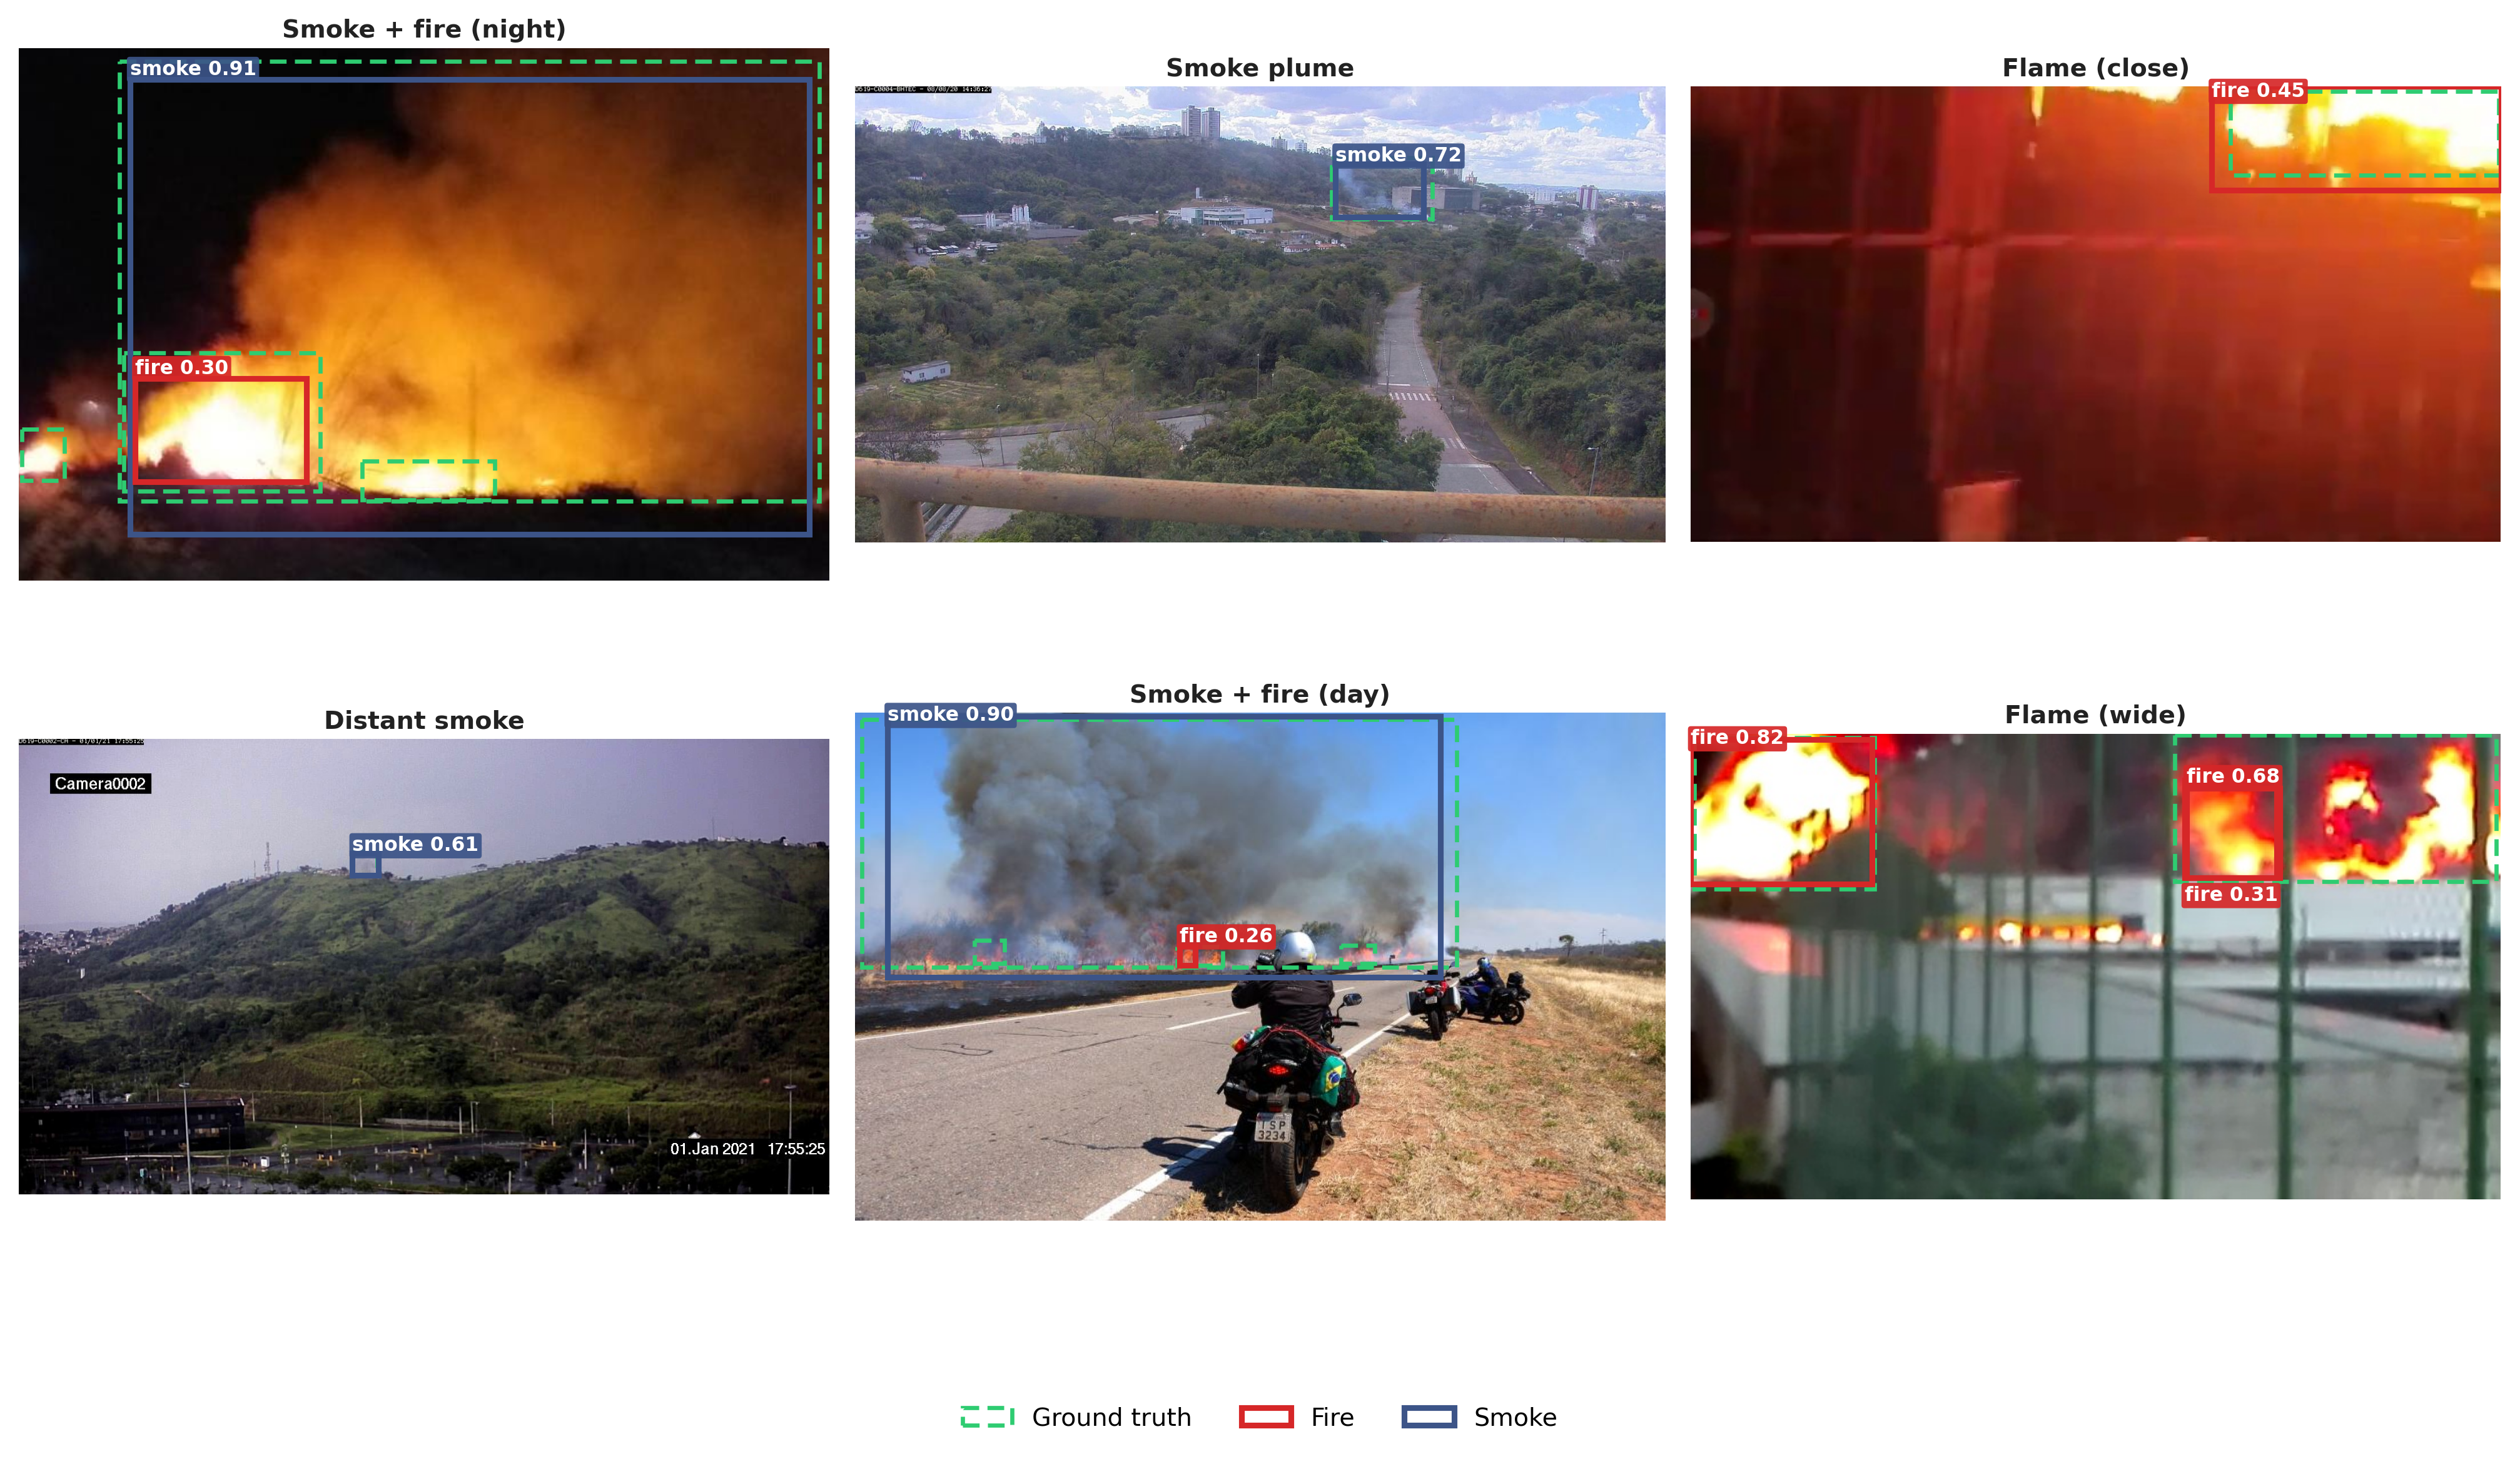
\includegraphics[width=\textwidth]{images/generated/fig_11_dfire_qualitative.png}
\caption{Qualitative detections from the trained YOLO26s (CLAHE) checkpoint (77.10\% mAP$_{50}$, top row of Table~\ref{tab:dfire_results}) on six real D-Fire test images spanning smoke-only, fire-only, combined, and small/distant hazard cases. Dashed green boxes are ground truth; solid coloured boxes are model predictions with confidence scores. Low-confidence and imperfectly localized predictions (e.g.\ the 0.26--0.45 confidence fire boxes) are shown as-is to illustrate genuine model behaviour rather than only best-case outputs.}
\label{fig:dfire_qualitative}
\end{figure}

Figure~\ref{fig:performance_benchmark} places the two evaluation tracks side by side: the independently trained D-Fire detectors and the scene-classification recovery of the joint prototype.

\begin{figure}[H]
\centering
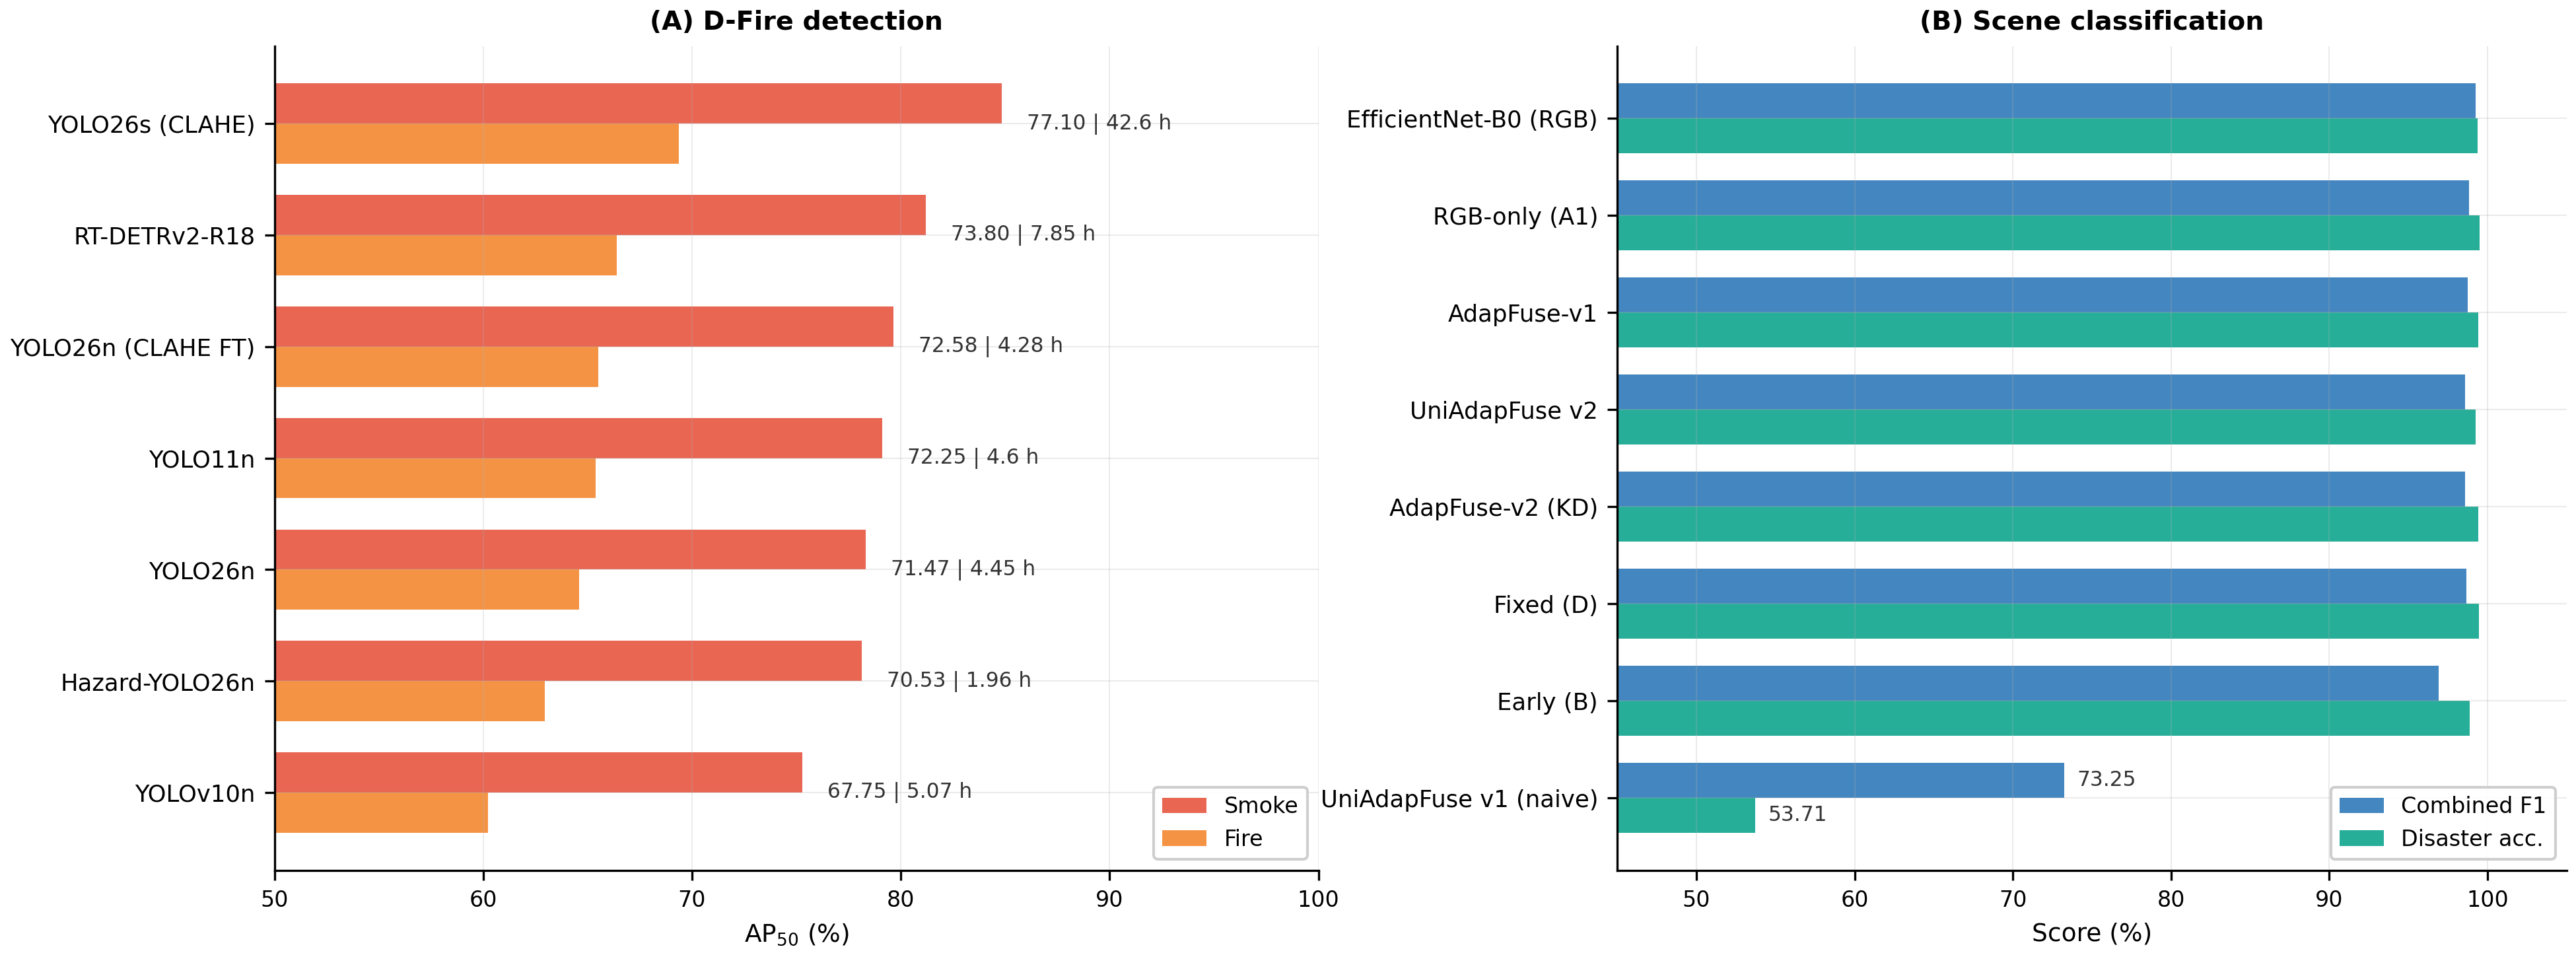
\includegraphics[width=\textwidth]{images/generated/fig_03_performance.png}
\caption{Two evaluation tracks: (A) independently trained D-Fire detectors with class-wise AP and wall-clock training time; (B) scene-classification recovery in the UniAdapFuse v2 prototype after gradient isolation. Numbers beside the bars in (A) give mAP$_{50}$ (\%) and training time. In (B), naive joint training (UniAdapFuse v1) falls to 53.71\% disaster accuracy, and stop-gradient isolation (v2) restores 99.26\% (+45.55\,pp). Panel B does not establish dense-detection quality: our v2 test log records detection $\mathrm{mAP}_{50}=0.0$.}
\label{fig:performance_benchmark}
\end{figure}

\section[Unified Perception Attempt: Classification Recovered, Detection Not]{Unified Perception Attempt: Negative Transfer Resolved for Classification but Not Detection}
\label{sec:uniadaptfuse}

\noindent\textbf{Summary of finding.} Naive joint training collapses disaster accuracy from 99.44\% to 53.71\%. Phased curriculum training and stop-gradient isolation recover classification to 98.57\% combined macro-F1, close to the standalone classifier (98.74\%), but the same saved checkpoint records a detection $\mathrm{mAP}_{50}$ of 0.0. The joint prototype therefore does not achieve joint perception, and all dense-detection results in this work (Section~\ref{sec:object_detection}) come from independently trained detectors on D-Fire, not from the unified architecture. Our artefacts do not identify the cause of the detection failure; candidate explanations include the small detection loss weight (0.2), the detection-head learning rate, or an error in the detection target or evaluation path, and diagnosing it is left to future work.

While standalone object detectors provide spatial bounding boxes, they lack global disaster scene context and victim presence estimation. To bridge this gap, \textbf{UniAdapFuse} couples multi-scale visual-thermal Feature Pyramid Networks (FPN) with the tri-modal classification backbone, connected via Top-Down Context Gates (TDCG) and Bottom-Up Spatial Guidance (BUSG)~\cite{perez2018film}.

\subsection{Curriculum Warmup and Stop-Gradient Isolation}

Naive joint training of global scene classification and dense bounding box regression (UniAdapFuse v1) suffers from catastrophic \textit{multi-task negative transfer}: disaster classification accuracy collapses from 99.44\% to 53.71\% because dense regression losses (CIoU and objectness) produce conflicting gradients that corrupt the shared visual backbone. 

UniAdapFuse v2 addresses this conflict on the classification side through three mechanisms: (1) \textit{Phased Curriculum Training}~\cite{bengio2009curriculum} with a 15-epoch classification-only warmup; (2) \textit{Stop-Gradient Isolation} (\texttt{.detach()}) applied to multi-scale pyramid feature maps before feeding the detection neck, ensuring detection gradients cannot backpropagate into the shared backbone; and (3) \textit{Differentiated Learning Rates} ($0.1\times$ backbone, $1.0\times$ classifier/bridge, $0.3\times$ detection head). Table~\ref{tab:uniadaptfuse_results} shows that classification is recovered while detection is not. Note that \texttt{.detach()} blocks detection gradients from reaching the shared backbone only; the detection neck and head still receive their own gradients, so the isolation mechanism by itself does not explain the zero $\mathrm{mAP}_{50}$.

\begin{table}[H]
\centering
\caption{UniAdapFuse scene-classification recovery ($n=10{,}951$ test rows). Standalone AdapFuse-v1 is the classification reference. UniAdapFuse v2 restores classification performance, but its recorded dense-detection $\mathrm{mAP}_{50}$ remains 0.0; producing prediction tensors is not equivalent to validated localization.}
\label{tab:uniadaptfuse_results}
\resizebox{\textwidth}{!}{%
\begin{tabular}{@{}lccccccc@{}}
\toprule
\textbf{Model} & \textbf{Architecture / Training Mechanism} & \textbf{Dis.\ F1} & \textbf{Dis.\ Acc} & \textbf{Vic.\ F1} & \textbf{Vic.\ Acc} & \textbf{Comb.\ F1} & \textbf{Det. mAP$_{50}$} \\
\midrule
AdapFuse-v1 (standalone) & Classification only baseline & 0.9913 & 0.9944 & 0.9836 & 0.9884 & 0.9874 & n/a \\
UniAdapFuse v1 (naive) & Naive Joint End-to-End Training & 0.5669 & 0.5371 & 0.8980 & 0.9306 & 0.7325 & n/a \\
\textbf{UniAdapFuse v2 (enhanced)} & \textbf{Joint graph + Gradient Isolation} & \textbf{0.9920} & \textbf{0.9926} & \textbf{0.9794} & \textbf{0.9856} & \textbf{0.9857} & \textbf{0.0000} \\
\midrule
\multicolumn{2}{l}{\textit{v2 Classification Recovery Gain over v1}} & \textbf{+42.51 pp} & \textbf{+45.55 pp} & \textbf{+8.14 pp} & \textbf{+5.50 pp} & \textbf{+25.32 pp} & n/a \\
\bottomrule
\end{tabular}%
}
\end{table}

UniAdapFuse v2 achieves \textbf{99.20\% disaster F1 and 98.57\% combined F1}, within 0.17 percentage points of the standalone classification reference. This demonstrates recovery of the classification branch after gradient isolation. However, our \texttt{uni\_adaptfuse\_v2\_test\_results.json} reports $\mathrm{mAP}_{50}=0.0$ for detection. Our evidence therefore does not establish usable joint localization or compatibility between the tasks; the independent D-Fire detector results in Section~\ref{sec:object_detection} remain the valid localization benchmark.

\section{Multimodal Scene-Prior and Reliability Benchmark (Row-Level Split)}
\label{sec:classification_benchmark}

The global scene classification stream is intended to provide a prior for the detection stream. In the current evidence, scene classification and the independently trained D-Fire detectors are validated separately; a working scene-conditioned detector is not established. All twenty-six classification configurations were evaluated on the row-level held-out test set ($n=10{,}951$). Table~\ref{tab:main_results} presents the complete comparison ranked by Combined F1.

\textbf{Metric definition.} Throughout this chapter, \emph{Combined F1} is the unweighted mean of the two task-level macro-F1 scores,
\begin{equation}
    \text{Combined F1} = \tfrac{1}{2}\left(\text{macro-F1}_{\text{disaster}} + \text{macro-F1}_{\text{victim}}\right),
\end{equation}
where disaster macro-F1 averages over the four disaster classes and victim macro-F1 over the two victim-presence classes. Macro averaging weights every class equally, so rare classes are not hidden by the natural test distribution, and the outer mean weights the two tasks equally.

\textbf{Interpretation caveat.} Every score in Table~\ref{tab:main_results} comes from the row-level split, which is not grouped by capture sequence, and from a corpus in which source identity and label are entangled (Section~\ref{sec:per_source}). Differences between configurations are therefore within-collection comparisons, not evidence of generalization to new flights, sensors or regions.

\begin{table}[H]
\centering
\caption{Master Performance Comparison of All Twenty-Six Multimodal Classification Models ($n=10{,}951$, natural distribution), globally ranked by Combined F1. All models trained on the Stratified Balanced Training Subset (49{,}276 samples, 25\% per class). These are row-level scores: the split is not grouped by capture sequence, so every value in this table is a within-collection estimate. Section~\ref{sec:grouped_split} reports the same architecture under a capture-group-aware split, where combined macro-F1 falls by 9.60 percentage points.}
\label{tab:main_results}
\resizebox{\textwidth}{!}{%
\begin{tabular}{@{}rllcccccc@{}}
\toprule
\textbf{Rank} & \textbf{Model / Experiment} & \textbf{Family / Type} & \textbf{Test Loss} & \textbf{Dis.\ F1} & \textbf{Vic.\ F1} & \textbf{Comb.\ F1} & \textbf{Dis.\ Acc} & \textbf{Vic.\ Acc} \\
\midrule
1 & \textbf{AdapFuse-v1 + EfficientNet-B0 (RGB)} & Visual Backbone & 0.0025 & 0.9923 & \textbf{0.9924} & \textbf{0.9924} & 0.9940 & \textbf{0.9947} \\
2 & \textbf{AdapFuse-v1 + MobileViT-XXS (RGB)} & Visual Backbone & 0.0103 & 0.9881 & 0.9916 & \textbf{0.9899} & 0.9931 & 0.9942 \\
3 & Baseline A1: RGB-Only & Unimodal Baseline & 0.0054 & 0.9924 & 0.9846 & 0.9885 & \textbf{0.9951} & 0.9891 \\
4 & AdapFuse-v1 + EfficientNet-B0 (Thermal) & Visual Backbone & 0.0095 & 0.9924 & 0.9837 & 0.9880 & 0.9950 & 0.9886 \\
5 & Ablation: No RUE (\texttt{ablation\_no\_rue}) & Component Ablation & 0.0094 & \textbf{0.9938} & 0.9812 & 0.9875 & \textbf{0.9957} & 0.9868 \\
6 & \textbf{AdapFuse-v1 (E): Base Teacher} & Proposed Method & \textbf{0.0020} & 0.9913 & 0.9836 & 0.9874 & 0.9944 & 0.9884 \\
7 & Ablation: No Nuisance Head & Component Ablation & 0.0092 & 0.9923 & 0.9821 & 0.9872 & 0.9942 & 0.9874 \\
8 & Intermediate Fixed Fusion (D) & Core Fusion Topology & 0.0059 & 0.9911 & 0.9828 & 0.9869 & 0.9947 & 0.9879 \\
9 & Late Fusion (C) & Core Fusion Topology & 0.0048 & 0.9916 & 0.9817 & 0.9867 & 0.9939 & 0.9871 \\
10 & AdapFuse-v1 + GDBlock & Audio Backbone & 0.0036 & 0.9888 & 0.9838 & 0.9863 & 0.9924 & 0.9886 \\
11 & AdapFuse-v2 KD Student (F) & Knowledge Distillation & 0.0035 & 0.9917 & 0.9805 & 0.9861 & 0.9944 & 0.9862 \\
12 & \textbf{UniAdapFuse v2 (Joint Cls + Det)} & Unified Multi-Task & n/a & 0.9920 & 0.9794 & \textbf{0.9857} & 0.9926 & 0.9856 \\
13 & RGB + Thermal Subset & Two-Sensor Subset & 0.0042 & 0.9870 & 0.9830 & 0.9850 & 0.9898 & 0.9880 \\
14 & RGB + Audio Subset & Two-Sensor Subset & 0.0021 & 0.9896 & 0.9802 & 0.9849 & 0.9942 & 0.9860 \\
15 & AdapFuse-v1 + Domain Prompts & Architecture Module & 0.0035 & 0.9885 & 0.9813 & 0.9849 & 0.9927 & 0.9869 \\
16 & AdapFuse-v2 KD + PANNS & Audio Backbone & 0.0041 & 0.9884 & 0.9813 & 0.9848 & 0.9924 & 0.9868 \\
17 & AdapFuse-v1 + Spatial Attention & Architecture Module & 0.0034 & 0.9874 & 0.9814 & 0.9844 & 0.9902 & 0.9869 \\
18 & Ablation: No Quality Tokens & Component Ablation & 0.0108 & 0.9881 & 0.9800 & 0.9840 & 0.9927 & 0.9858 \\
19 & Ablation: No Cross-Attention & Component Ablation & 0.0076 & 0.9894 & 0.9785 & 0.9839 & 0.9925 & 0.9848 \\
20 & AdapFuse-v1 + PANNS & Audio Backbone & 0.0038 & 0.9858 & 0.9792 & 0.9825 & 0.9907 & 0.9853 \\
21 & Ablation: No GRU Temporal Cell & Component Ablation & 0.0102 & 0.9863 & 0.9765 & 0.9814 & 0.9901 & 0.9833 \\
22 & Thermal + Audio Subset & Two-Sensor Subset & 0.0058 & 0.9880 & 0.9730 & 0.9805 & 0.9912 & 0.9809 \\
23 & Thermal-only (A2) & Unimodal Baseline & 0.0102 & 0.9802 & 0.9684 & 0.9743 & 0.9838 & 0.9774 \\
24 & Early Fusion (B) & Core Fusion Topology & 0.0126 & 0.9832 & 0.9554 & 0.9693 & 0.9890 & 0.9685 \\
25 & UniAdapFuse v1 (Naive Joint) & Unified Multi-Task & 0.0137 & 0.5669 & 0.8980 & 0.7325 & 0.5371 & 0.9306 \\
26 & Audio-only (A3) & Unimodal Baseline & 0.1325 & 0.3820 & 0.4365 & 0.4093 & 0.7169 & 0.7746 \\
\bottomrule
\end{tabular}%
}
\end{table}

\textbf{Fusion versus the RGB-only baseline.} Table~\ref{tab:main_results} does not show a fusion advantage on this split. The RGB-only baseline A1 (98.85\% combined F1) scores 0.11 points above AdapFuse-v1 (98.74\%), and the no-RUE ablation (98.75\%) matches the full model, so reliability-aware fusion does not raise row-level F1 above the RGB stream alone. AdapFuse-v1's advantage over A1 is limited to test loss (0.0020 against 0.0054). The two configurations ranked above A1 are AdapFuse-v1 with a stronger RGB backbone. Section~\ref{sec:unimodal_backbones} trains RGB-only models with the same backbones: RGB-only MobileViT-XXS (98.99\%) equals AdapFuse-v1 + MobileViT-XXS (98.99\%), and RGB-only EfficientNet-B0 (98.88\%) is 0.36 points below AdapFuse-v1 + EfficientNet-B0 (99.24\%), with the unimodal run limited to 12 epochs. These gaps are small single-seed differences. With the pseudo-thermal map derived from RGB and the audio label-matched, the fused inputs carry little information beyond the RGB frame, so a fusion benefit could only be tested with independent sensors.

\subsection{Unimodal Backbone Comparison}
\label{sec:unimodal_backbones}

To separate the effect of the backbone from the effect of fusion, each single-modality baseline was trained with three backbones: the original A1--A3 encoder and two alternatives. These models were trained through the same AdapFuse-UAV pipeline as the fused models, with the same classifier head, focal loss, balanced training subset, augmentation, synthetic corruption, mixed precision, early stopping and row-level test set ($n=10{,}951$) as Table~\ref{tab:main_results}. Every backbone was therefore trained inside the pipeline twice, once as a unimodal encoder and once as an AdapFuse-v1 encoder, so the two can be compared directly. Tables~\ref{tab:unimodal_rgb}--\ref{tab:unimodal_audio} report one table per modality. To bound training time, the new visual runs used a 12-epoch budget (2 warm-up epochs, cosine schedule, early-stopping patience 5); the original A1--A3 runs used a 50-epoch budget. The comparison therefore favours the original encoders, and every result is a single seed. Dense detection is evaluated on RGB only; those results are in Table~\ref{tab:dfire_results}.

\begin{table}[H]
\centering
\caption{RGB-only scene classification with three backbones (row-level test set, $n=10{,}951$). Params counts the full unimodal model, including both classifier heads. Epochs shows epochs run / epoch budget. Best value per column in bold.}
\label{tab:unimodal_rgb}
\resizebox{\textwidth}{!}{%
\begin{tabular}{@{}llcccccccc@{}}
\toprule
\textbf{Model} & \textbf{Backbone} & \textbf{Params} & \textbf{Epochs} & \textbf{Test Loss} & \textbf{Dis.\ F1} & \textbf{Vic.\ F1} & \textbf{Comb.\ F1} & \textbf{Dis.\ Acc} & \textbf{Vic.\ Acc} \\
\midrule
A1 & MobileNetV3-Small & 1.22M & 50 / 50 & \textbf{0.0054} & \textbf{0.9924} & 0.9846 & 0.9885 & \textbf{0.9951} & 0.9891 \\
A1b & EfficientNet-B0 & 4.66M & 12 / 12 & 0.0125 & 0.9887 & 0.9889 & 0.9888 & 0.9923 & 0.9922 \\
A1c & MobileViT-XXS & \textbf{1.12M} & 12 / 12 & 0.0105 & 0.9882 & \textbf{0.9915} & \textbf{0.9899} & 0.9921 & \textbf{0.9941} \\
\bottomrule
\end{tabular}%
}
\end{table}

\begin{table}[H]
\centering
\caption{Pseudo-thermal-only scene classification with three backbones (1-channel input; row-level test set). The input is derived from RGB, not measured LWIR. A2 stopped early at epoch 36 of 50.}
\label{tab:unimodal_thermal}
\resizebox{\textwidth}{!}{%
\begin{tabular}{@{}llcccccccc@{}}
\toprule
\textbf{Model} & \textbf{Backbone} & \textbf{Params} & \textbf{Epochs} & \textbf{Test Loss} & \textbf{Dis.\ F1} & \textbf{Vic.\ F1} & \textbf{Comb.\ F1} & \textbf{Dis.\ Acc} & \textbf{Vic.\ Acc} \\
\midrule
A2 & ResNet-18 (1-ch) & 11.43M & 36 / 50 & \textbf{0.0102} & 0.9802 & 0.9684 & 0.9743 & 0.9838 & 0.9774 \\
A2b & EfficientNet-B0 (1-ch) & 4.66M & 12 / 12 & 0.0126 & \textbf{0.9927} & \textbf{0.9794} & \textbf{0.9860} & \textbf{0.9934} & \textbf{0.9855} \\
A2c & MobileViT-XXS (1-ch) & \textbf{1.12M} & 12 / 12 & 0.0117 & 0.9905 & 0.9788 & 0.9846 & 0.9918 & 0.9851 \\
\bottomrule
\end{tabular}%
}
\end{table}

\begin{table}[H]
\centering
\caption{Audio-only scene classification with three backbones (log-mel input from label-matched ESC-50 clips; row-level test set). A3b and A3c stopped early (budget 40 epochs) and produced identical test metrics; see text. They are degenerate solutions, not evidence that the backbone improves audio recognition.}
\label{tab:unimodal_audio}
\resizebox{\textwidth}{!}{%
\begin{tabular}{@{}llcccccccc@{}}
\toprule
\textbf{Model} & \textbf{Backbone} & \textbf{Params} & \textbf{Epochs} & \textbf{Test Loss} & \textbf{Dis.\ F1} & \textbf{Vic.\ F1} & \textbf{Comb.\ F1} & \textbf{Dis.\ Acc} & \textbf{Vic.\ Acc} \\
\midrule
A3 & AudioCNN (scratch) & 0.11M & 50 / 50 & \textbf{0.1325} & 0.3820 & 0.4365 & 0.4093 & \textbf{0.7169} & \textbf{0.7746} \\
A3b & PANNS-CNN6$^\dagger$ & 1.62M & 24 / 40 & 0.2610 & 0.4153 & 0.5777 & 0.4965 & 0.5673 & 0.6163 \\
A3c & AudioCNN + GDBlock & \textbf{0.07M} & 25 / 40 & 0.2625 & 0.4153 & 0.5777 & 0.4965 & 0.5673 & 0.6163 \\
\bottomrule
\multicolumn{10}{@{}l}{\footnotesize $^\dagger$Only 8 of the encoder's 20 weight tensors were loaded from the AudioSet checkpoint; the encoder is partially pretrained.}
\end{tabular}%
}
\end{table}

\textbf{RGB.} The three RGB backbones fall within 0.14 combined-F1 points of each other (98.85--98.99\%). MobileViT-XXS gives the best combined F1 and victim-presence F1 with the fewest parameters, while MobileNetV3-Small keeps the best disaster F1 and test loss after a four-times longer training budget. RGB-only classification is at its ceiling on this split, so a stronger RGB encoder adds little.

\textbf{Pseudo-thermal.} Changing the backbone matters more here: EfficientNet-B0 raises combined F1 from 97.43\% (ResNet-18) to 98.60\% in 12 epochs, and MobileViT-XXS reaches 98.46\% with one-tenth of ResNet-18's parameters. MobileViT-XXS validation F1 was still rising at epoch 12 (97.28\% at epoch 11), so its score is limited by the training budget. The best pseudo-thermal model remains 0.39 points below the best RGB model, which is expected because the map is computed from the same RGB frame and discards colour.

\textbf{Audio.} Neither alternative encoder learned a useful audio classifier. PANNS-CNN6 and GDBlock produced exactly the same test metrics to every reported digit, their training accuracy plateaued at 55.7\% from the first epochs, and their training loss hardly changed. Two different architectures reaching identical predictions indicates a shared degenerate decision rule that does not depend on audio content. Their higher combined F1 than A3 (49.65\% against 40.93\%) is therefore not an improvement: A3 has higher accuracy on both tasks and a lower test loss. All three audio results reflect label-matched ESC-50 clips that are not synchronised with the visual scene (Section~\ref{sec:backbone_variants}), so they measure that pairing, not UAV acoustic sensing.

\begin{table}[H]
\centering
\caption{Accuracy against cost for the trained visual backbones (combined F1, \%, row-level test set). Cost columns are from Table~\ref{tab:backbone_candidates}. The fused columns give AdapFuse-v1 with that backbone in the named stream; the base AdapFuse-v1 (98.74\%) uses MobileNetV3-Small for RGB and ResNet-18 for pseudo-thermal. $^\dagger$Lower bound. -- = not trained.}
\label{tab:backbone_accuracy_cost}
\resizebox{\textwidth}{!}{%
\begin{tabular}{@{}lcccccc@{}}
\toprule
\textbf{Backbone} & \textbf{GMACs} & \textbf{Params (M)} & \textbf{RGB-only} & \textbf{Thermal-only} & \textbf{Fused (RGB stream)} & \textbf{Fused (thermal stream)} \\
\midrule
MobileNetV3-Small & \textbf{0.06} & 0.93 & 98.85 & -- & 98.74 & -- \\
MobileViT-XXS & 0.30$^\dagger$ & 0.95 & \textbf{98.99} & 98.46 & 98.99 & -- \\
EfficientNet-B0 & 0.39 & 4.01 & 98.88 & \textbf{98.60} & \textbf{99.24} & \textbf{98.80} \\
ResNet-18 & 1.81 & 11.18 & -- & 97.43 & -- & 98.74 \\
\bottomrule
\end{tabular}%
}
\end{table}

Table~\ref{tab:backbone_accuracy_cost} gives the outcome of the selection in Section~\ref{sec:backbone_selection}. For RGB, the cheapest encoder is within 0.14 points of the best, so MobileNetV3-Small remains a reasonable default at one-fifth of MobileViT-XXS's MACs. For pseudo-thermal, the over-budget ResNet-18 is both the most expensive and the least accurate choice; EfficientNet-B0 is 1.17 points better at 21\% of its MACs, which makes it the better default for that stream.

\textbf{Matched-backbone fusion comparison.} With the backbone held fixed, fusion adds 0.36 combined-F1 points for EfficientNet-B0 on RGB (99.24\% against 98.88\%), nothing for MobileViT-XXS on RGB (98.99\% for both), and 0.20 points for EfficientNet-B0 on the pseudo-thermal stream (98.80\% against 98.60\%). The unimodal runs had a shorter budget (12 epochs against 22, 15 and 7 epochs run for the fused models), so these small gaps do not show that fusion helps; they are consistent with the conclusion above that the fused inputs add little beyond the RGB frame.

\subsection{Comparison with Published Results on Public Benchmarks}
\label{sec:public_benchmark_results}

The row-level scores above cannot be compared with published work, because our corpus merges six sources and splits them at random. To obtain comparable numbers, three models were retrained through the same AdapFuse-UAV pipeline under the published protocols of two public datasets (Section~\ref{sec:public_benchmarks_related}): RGB-only MobileNetV3-Small (A1), RGB-only EfficientNet-B0 (A1b) and AdapFuse-v1 with RGB and its derived pseudo-thermal map (audio absent). All used ImageNet-pretrained encoders, focal loss, the same augmentation and synthetic corruption, and model selection on the validation split; each is a single seed.

\textbf{AIDER protocol.} The 6{,}433-image AIDER subset was split per class with exactly the train/validation/test counts of Lee et al.~\cite{lee2023wattefnet} (3{,}207 / 753 / 2{,}473; five classes, 71\% of test images normal). Models trained for up to 30 epochs without resampling.

\begin{table}[H]
\centering
\caption{AIDER subset, 4:1:2 protocol (2{,}473 test images, five classes). Published rows are copied from Lee et al.~\cite{lee2023wattefnet}, who trained every model from scratch for 300 epochs and do not state the F1 averaging; our rows use ImageNet-pretrained encoders and report macro-F1. Params counts the full model.}
\label{tab:public_aider}
\resizebox{\textwidth}{!}{%
\begin{tabular}{@{}llccc@{}}
\toprule
\textbf{Model} & \textbf{Source} & \textbf{Params (M)} & \textbf{F1 (\%)} & \textbf{Accuracy (\%)} \\
\midrule
EfficientNet & Lee et al.~\cite{lee2023wattefnet} & 3.50 & 80.0 & -- \\
MobileNetV2 & Lee et al.~\cite{lee2023wattefnet} & 2.28 & 81.0 & -- \\
EmergencyNet~\cite{kyrkou2020emergencynet} & Lee et al.~\cite{lee2023wattefnet} & 0.09 & 83.1 & -- \\
WATT-EffNet-3-6 & Lee et al.~\cite{lee2023wattefnet} & 0.69 & 88.5 & -- \\
\midrule
RGB-only MobileNetV3-Small (A1) & Ours & 1.22 & 93.02 & 96.48 \\
RGB-only EfficientNet-B0 (A1b) & Ours & 4.67 & \textbf{94.00} & \textbf{97.01} \\
AdapFuse-v1 (RGB + pseudo-thermal) & Ours & 12.94 & 91.86 & 95.79 \\
\bottomrule
\end{tabular}%
}
\end{table}

All three of our models exceed the published AIDER F1 scores (Table~\ref{tab:public_aider}), with RGB-only EfficientNet-B0 at 94.00\% macro-F1 against 88.5\% for WATT-EffNet. The comparison is not like-for-like: our encoders start from ImageNet weights, whereas Lee et al.\ trained from scratch to study lightweight design, and the F1 averaging of the published table is not stated. The margin is therefore evidence that ImageNet transfer inside our pipeline is effective on AIDER, not that our architectures are better designed. Fusion again does not help: AdapFuse-v1 is 2.14 points below RGB-only EfficientNet-B0, because the pseudo-thermal map carries no information beyond the RGB frame.

\textbf{FLAME protocol.} Models trained on the official FLAME training folder (39{,}375 frames from a Matrice 200 with a Zenmuse X4S), with a random 20\% of it held out for validation as in the original paper, and were tested on the official test folder (8{,}617 frames from a Phantom 3)~\cite{shamsoshoara2021aerial}. Training was limited to 10 epochs.

\begin{table}[H]
\centering
\caption{FLAME fire/no-fire classification, official protocol (8{,}617 test frames from a different drone and camera than training). Validation F1 is on the held-out 20\% of the training folder (same drone). The published row is from Shamsoshoara et al.~\cite{shamsoshoara2021aerial}. $^\ast$Binary cross-entropy; our losses are focal loss and are not comparable.}
\label{tab:public_flame}
\resizebox{\textwidth}{!}{%
\begin{tabular}{@{}lccccc@{}}
\toprule
\textbf{Model} & \textbf{Best epoch} & \textbf{Val.\ F1 (\%)} & \textbf{Test F1 (\%)} & \textbf{Test Acc.\ (\%)} & \textbf{Test Loss} \\
\midrule
Xception~\cite{shamsoshoara2021aerial} (published) & -- & -- & -- & 76.23 & 0.7414$^\ast$ \\
\midrule
Ours: RGB-only MobileNetV3-Small & 1 & 99.86 & 62.76 & 69.41 & 0.1800 \\
Ours: RGB-only EfficientNet-B0 & 1 & 99.92 & \textbf{82.85} & \textbf{83.72} & 0.0856 \\
Ours: AdapFuse-v1 (RGB + pseudo-th.) & 9 & 99.96 & 72.93 & 75.53 & 0.1332 \\
\bottomrule
\end{tabular}%
}
\end{table}

Table~\ref{tab:public_flame} shows the effect this thesis has to contend with. Every model scores 99.86--99.96\% F1 on validation frames from the training drone and 62.76--82.85\% on the test drone, a drop of 17 to 37 points. RGB-only EfficientNet-B0 reaches 83.72\% test accuracy, 7.49 points above the published Xception result; MobileNetV3-Small (69.41\%) and AdapFuse-v1 (75.53\%) fall below it. Because the in-domain validation split is saturated from the first epoch, it cannot guide model selection for the new camera: both RGB-only runs kept their epoch-1 checkpoints and stopped early. These results support the conclusion of Section~\ref{sec:grouped_split}: scores on frames from the same capture as training are near ceiling and overstate performance on new hardware. They also show that on a genuine cross-camera test the stronger backbone matters more than fusion with an RGB-derived map.

\subsection{Row-Level False Positives and Probabilistic Calibration}
\label{sec:adaptfuse_extended}

Table~\ref{tab:adaptfuse_extended} reports extended metrics for AdapFuse-v1, including our averages of the \textit{Reliability and Uncertainty Estimator (RUE)} gates. Because the nuisance branch is unsupervised and the gates are not trained against degradation targets, these values describe the fitted model; they do not measure the effect of either component.

\begin{table}[H]
\centering
\caption{AdapFuse-v1 Extended Evaluation Metrics ($n=10{,}951$ test samples)}
\label{tab:adaptfuse_extended}
\begin{tabular}{@{}ll>{\raggedright\arraybackslash}p{6.0cm}@{}}
\toprule
\textbf{Metric} & \textbf{Value} & \textbf{Operational Significance} \\
\midrule
Disaster F1 (macro)    & 0.9913 & 4-class multi-disaster categorization \\
Disaster Accuracy      & 0.9944 & Evaluated on natural distribution \\
Disaster Precision     & 0.9870 & High confidence in positive alerts \\
Disaster Recall        & 0.9957 & Extremely low miss rate on active hazards \\
Victim F1 (macro)      & 0.9836 & Binary survivor presence detection \\
Victim Accuracy        & 0.9884 & \\
\midrule
\textbf{False Positive Rate (FPR)} & \textbf{0.0073} & Row-level scene-classification FPR \\
\textbf{Expected Calibration Error (ECE)} & \textbf{0.0337} & Calibration statistic on the row-level split \\
\textbf{Test Loss (Focal)} & \textbf{0.0020} & Lowest across all evaluated architectures \\
\midrule
Avg Reliability: RGB$^\dagger$   & 0.972  & $\approx$1.0 on every row with RGB; unchanged under corruption \\
Avg Reliability: Pseudo-thermal$^\dagger$ & 0.972 & $\approx$1.0 on every row with the map; unchanged under corruption \\
Avg Reliability: Audio$^\dagger$ & \textbf{0.006}  & $\approx$0.011 on rows with audio; label-matched audio largely ignored \\
\midrule
Total Parameters       & 12.94M & Compact multi-branch footprint \\
Inference Latency (batch=1) & 14.26 ms & 70.1 FPS on workstation RTX 5090 \\
\bottomrule
\end{tabular}

\vspace{1mm}
\parbox{0.95\textwidth}{\footnotesize $^\dagger$Means over all 10{,}951 test rows. The model sets a gate to zero whenever its modality is missing, and the averaging script (\texttt{reliability\_analysis.py}) includes those rows. 0.972 equals the fraction of test rows that have RGB and pseudo-thermal inputs (10{,}646/10{,}951 = 0.9721), so both image gates sit at $\approx$1.0 on every row that has the input. The audio mean of 0.006 over all rows corresponds to $\approx$0.011 over the 5{,}781 rows that have an audio clip.}
\end{table}

\textbf{Observed row-level false-positive rate (0.73\%):}
Our evaluation reports a 0.73\% false-positive rate for scene classification on the row-level test split. This is not an operational field false-alarm study and cannot be causally attributed to the NuisanceAwareHead, because our trainer passes \texttt{nuisance\_gt=None} and its nuisance loss is zero.

\textbf{Learned modality gates:}
The reported averages (audio 0.006, image streams 0.972) include rows whose gate is forced to zero because the modality is missing. Restricted to rows that have each input, the row-level model's RGB and pseudo-thermal gates are saturated at $\approx$1.0 and its audio gate is $\approx$0.011; the RUE is therefore effectively passing both image streams through unchanged and switching audio off. In this run the learned representation largely ignores the label-matched ESC-50 channel, which is the expected outcome: because each clip is paired with visual rows by shared label rather than recorded with them, the audio carries no information about the specific scene beyond what the label already implies. The low audio gate is therefore a consequence of the data construction, not evidence of learned reliability estimation. It is also not a stable property of the architecture: the grouped-split retraining (Section~\ref{sec:grouped_gates}) converges to the opposite audio gate. Likewise, the RGB and pseudo-thermal gates remain essentially constant across all tested corruption severities (Section~\ref{sec:robustness_stress_test}). In our model, the RUE behaves as a learned, largely input-independent feature weighting rather than as a dynamic reliability estimator; corruption-sensitive gating would require training with explicit degradation targets and evaluating gate response against measured degradation, neither of which is present here.

\subsection{Per-Module Latency Breakdown}

Table~\ref{tab:latency_profile} breaks down the 14.26\,ms total inference latency of AdapFuse-v1 by module, measured at batch size 1 on an NVIDIA RTX 5090 (32\,GB VRAM) (establishing the computational efficiency baseline prior to physical embedded edge deployment in future work).

\begin{table}[H]
\centering
\caption{Per-Module Inference Latency Breakdown for AdapFuse-v1 (batch=1, Workstation GPU)}
\label{tab:latency_profile}
\begin{tabular}{@{}lrr@{}}
\toprule
\textbf{Module} & \textbf{Latency (ms)} & \textbf{\% of Total Pipeline} \\
\midrule
RGB Backbone (MobileNetV3-Small) & 6.37 & 44.7\% \\
Thermal Backbone (ResNet-18)     & 5.17 & 36.3\% \\
Audio Backbone (AudioCNN)        & 0.47 &  3.3\% \\
Feature Projectors (3 streams)   & 0.30 &  2.1\% \\
Quality Token Heads              & 0.32 &  2.2\% \\
\textbf{Reliability and Uncertainty Estimator (RUE)} & \textbf{0.85} & \textbf{6.0\%} \\
Cross-Modal Attention Layer      & 0.22 &  1.5\% \\
Temporal GRU Cell                & 0.19 &  1.3\% \\
NuisanceAwareHead                & 0.37 &  2.6\% \\
\midrule
\textbf{Total Inference Pipeline} & \textbf{14.26} & \textbf{100.0\%} \\
\bottomrule
\end{tabular}
\end{table}

The feature extractors (RGB, pseudo-thermal, and audio backbones) account for 84.2\% of the measured execution time. The RUE, attention, GRU, and nuisance branch together add 1.63\,ms, with gate computation requiring 0.85\,ms (6.0\%). This profiles implementation overhead on the workstation GPU; it does not establish that the learned gates respond dynamically to degradation.

\textbf{Measurement scope.} All latency figures in this section were measured on an NVIDIA RTX 5090 workstation GPU (32\,GB VRAM), whose power draw far exceeds the $\leq$15\,W embedded payload targeted in Section~\ref{sec:tech_requirements}. They are not estimates of on-board UAV latency or power. Latency, power and thermal behaviour on an embedded accelerator, with and without INT8 quantisation, have not been measured and remain future work.

\section{Leakage-Resistant Grouped-Split Evaluation}
\label{sec:grouped_split}

Every result reported so far uses the row-level stratified split described in Section~\ref{sec:dataset_split}, which does not group by source video, flight, or near-duplicate sequence. To quantify how much of the near-ceiling performance depends on that choice, a capture-group-aware split was rebuilt and AdapFuse-v1 was retrained on it from scratch.

\textbf{Grouped split construction.} The 72{,}997 rows were repartitioned into 50{,}845 training, 11{,}055 validation, and 11{,}097 test rows under a capture-group constraint, yielding 9{,}267 / 2{,}003 / 2{,}002 disjoint capture groups. FLAME does not expose true video or flight identifiers in its released files, so its frames are blocked in contiguous runs of 250 as an explicit adjacent-frame proxy; C2A augmentations and SARD Roboflow variants are grouped by original-image identity; ESC-50 folds 1--3, 4 and 5 are assigned to train, validation and test respectively, and visual rows are re-paired only with clips from their own partition. The generated split contains zero capture-group overlap and zero ESC-50 path overlap across the three partitions.

\textbf{Training recipe differences.} The grouped retraining was not a like-for-like repeat of the row-level run. Our run configuration (\texttt{resolved\_config.yaml}) shows that it was trained with batch size 2 instead of 16, and with class balancing disabled (\texttt{use\_balanced: false}), i.e.\ on the 50{,}845 unbalanced grouped training rows (46.7\% fire/smoke, 4.0\% other hazard) rather than on a Stratified Balanced Subset. Optimiser, learning-rate schedule, epochs, early stopping and missing-modality dropout were unchanged. Consequently, the difference between the two columns of Table~\ref{tab:grouped_comparison} combines three effects (the split, the class balance of the training data, and the batch size), and the present runs cannot separate them. A controlled comparison requires retraining on the grouped split with the row-level recipe (balanced subset, batch size 16), or retraining on the row-level split with the grouped recipe.

\subsection{Aggregate Effect of the Grouped Retraining}

Table~\ref{tab:grouped_comparison} compares AdapFuse-v1 under the two split regimes.

\begin{table}[H]
\centering
\caption{AdapFuse-v1 under row-level versus capture-group-aware splitting. Both columns use the same architecture, but the training recipe also differs (batch size 16 vs.\ 2; Stratified Balanced Subset vs.\ unbalanced grouped training rows; see text), so $\Delta$ is not attributable to the split alone. The grouped column is a single completed training seed (see the note below the table). AdapFuse-v1 is a classification-only model, so detection $\mathrm{mAP}_{50}$ does not apply to either column.}
\label{tab:grouped_comparison}
\begin{tabular}{@{}lccr@{}}
\toprule
\textbf{Metric} & \textbf{Row-level split} & \textbf{Grouped split} & \textbf{$\Delta$} \\
                & ($n=10{,}951$)          & ($n=11{,}097$)         &                    \\
\midrule
Disaster macro-F1   & 0.9913 & 0.8485 & $-14.28$ pp \\
Victim macro-F1     & 0.9836 & 0.9343 & $-4.93$ pp \\
\textbf{Combined macro-F1} & \textbf{0.9874} & \textbf{0.8914} & $\mathbf{-9.60}$ \textbf{pp} \\
Disaster accuracy   & 0.9944 & 0.8905 & $-10.39$ pp \\
Victim accuracy     & 0.9884 & 0.9530 & $-3.54$ pp \\
Test focal loss     & 0.0020 & 0.1462 & $\times 73$ \\
Detection $\mathrm{mAP}_{50}$ & n/a & n/a & n/a \\
\bottomrule
\end{tabular}

\vspace{2mm}
\parbox{\textwidth}{\footnotesize \textbf{Note on replication (single-seed result).} Only one of three launched seeds produced a usable result, so the grouped figures are single-point estimates with no confidence interval. Three training seeds were launched against this split. Seed~42 (reported above) completed 49 epochs with valid validation and selected its checkpoint at epoch~45. Seed~41 completed 50 epochs, but its validation metrics collapsed to exactly 1.0000 on all four measures for sixteen consecutive epochs (22--37, validation loss pinned at 0.0012--0.0013) before recovering; its best-checkpoint selector fired inside that window, so its reported test score of 0.8766 combined macro-F1 reflects an arbitrarily selected epoch-22 checkpoint rather than a converged best model, and it is excluded from the table. Seed~43 halted at epoch~12 of 50 and has no test evaluation. All three runs used the identical partition, so they measure training-initialisation variance only and would not in any case bound variance due to the grouping itself. A corrected multi-seed interval is required before a confidence range is claimed.}
\end{table}

The grouped retraining scores 9.60 percentage points lower in combined macro-F1. The loss is asymmetric across tasks: victim-presence classification degrades by 4.93 pp, while disaster classification degrades by 14.28 pp and the test focal loss rises by roughly two orders of magnitude. Adjacent-frame memorisation would produce this pattern, because the disaster label is the one most strongly tied to which source video a frame came from. It is not the only explanation. The grouped model was trained without class balancing, and its weakest disaster classes are the two rare ones (collapse/flood F1 0.824, other hazard F1 0.765, against 0.899 and 0.906 for clean and fire/smoke), which is also what an imbalanced training set would produce. The much smaller batch size may add further differences. The 9.60-point figure should therefore be read as the combined effect of the grouped split and the recipe changes described above, not as a clean measurement of leakage.

The row-level figures reported elsewhere in this chapter should still be read as \emph{within-collection} performance, since the row-level split demonstrably places frames from the same capture sequences on both sides of the partition. The grouped figure is a more conservative estimate of behaviour on unseen capture sequences, but it is not a controlled one.

\subsection{Learned Gates in the Grouped Retraining}
\label{sec:grouped_gates}

The grouped run's saved per-row predictions (\texttt{test\_predictions.csv}) also record the three RUE gates, and they differ sharply from the row-level model. Joining them with the modality-presence flags of the grouped test metadata gives the following picture. Gates for missing modalities are exactly zero in both runs, as the model's presence mask requires.
\begin{itemize}
    \item \textbf{Audio:} the gate is 1.000 on all 5{,}982 test rows that have an audio clip, whereas the row-level model's audio gate is $\approx$0.011 on rows with audio. The two runs therefore learned opposite treatments of the same label-matched channel.
    \item \textbf{Pseudo-thermal:} on the 10{,}697 rows that have a pseudo-thermal map, the gate is bimodal (above 0.99 on 53.8\% of rows and below 0.01 on 43.5\%) and is switched off on 59.7\% of FLAME rows but only 1.4\% of C2A rows. In the excluded seed~41 run the pseudo-thermal gate is zero on every row.
    \item \textbf{RGB:} the gate is above 0.99 on 93.7\% of rows with RGB, close to the saturated behaviour of the row-level model.
\end{itemize}
Three conclusions follow. First, the gates are saturated at 0 or 1 in both runs, so the RUE behaves as a learned on/off switch per modality rather than as a graded reliability estimate. Second, which modalities are switched on depends on the training run: the row-level finding that ``the model ignores audio'' does not reproduce under the grouped retraining, so it should be read as a property of that single run, not of the architecture. Third, the pseudo-thermal gate in the grouped run varies strongly by source, which is consistent with the gate responding to dataset identity rather than to input quality. None of these runs supervises the gates with degradation targets, so none of them tests reliability estimation.

\subsection{Per-Source Decomposition and Source--Label Confounding}
\label{sec:per_source}

Table~\ref{tab:grouped_per_source} decomposes the same grouped-split predictions by originating dataset and lists which label values actually occur in each source's test rows.

\begin{table}[H]
\centering
\caption{Grouped-split test performance decomposed by source dataset (AdapFuse-v1, seed~42, $n=11{,}097$), recomputed from our \texttt{test\_predictions.csv}. ``Saved F1'' is the value written by the evaluation script, which averages over \emph{all} four disaster and both victim classes with \texttt{zero\_division=0}; classes that do not occur in a source therefore contribute an F1 of zero and cap the score (e.g.\ at 0.50 for a single-class victim source). ``Present-class F1'' averages only over classes that occur in that source. Victim-presence classes: 0 = no person visible, 1 = person visible.}
\label{tab:grouped_per_source}
\resizebox{\textwidth}{!}{%
\begin{tabular}{@{}lrllcccccc@{}}
\toprule
& & \multicolumn{2}{c}{\textbf{Classes present}} & \multicolumn{2}{c}{\textbf{Accuracy}} & \multicolumn{2}{c}{\textbf{Saved F1 (all classes)}} & \multicolumn{2}{c}{\textbf{Present-class F1}} \\
\cmidrule(lr){3-4} \cmidrule(lr){5-6} \cmidrule(lr){7-8} \cmidrule(lr){9-10}
\textbf{Source} & \textbf{$n$} & \textbf{Disaster} & \textbf{Victim} & \textbf{Dis.} & \textbf{Vic.} & \textbf{Dis.} & \textbf{Vic.} & \textbf{Dis.} & \textbf{Vic.} \\
\midrule
AIDER    &    965  & 0,1,2,3 & 0 only & 0.8415 & 0.5720 & 0.7637 & 0.3639 & 0.7637 & 0.7278 \\
C2A      & 1{,}535 & 1,2,3   & 1 only & 0.8169 & 0.9590 & 0.6326 & 0.4895 & 0.8435 & 0.9790 \\
FLAME    & 7{,}244 & 0,1     & 0 only & 0.8961 & 0.9994 & 0.4467 & 0.4999 & 0.8933 & 0.9997 \\
ESC-50   &    400  & 0,1     & 0 only & 0.9750 & 1.0000 & 0.3718 & 0.5000 & 0.7436 & 1.0000 \\
SARD     &    863  & 0 only  & 1 only & 0.9977 & 0.9930 & 0.2497 & 0.4983 & 0.9988 & 0.9965 \\
FireNet  &     90  & 1 only  & 0 only & 0.8222 & 0.6000 & 0.2256 & 0.3750 & 0.9024 & 0.7500 \\
\midrule
\textbf{Aggregate} & \textbf{11{,}097} & 0,1,2,3 & 0,1 & 0.8905 & 0.9530 & 0.8485 & 0.9343 & 0.8485 & 0.9343 \\
\bottomrule
\end{tabular}%
}
\end{table}

\textbf{The low saved per-source F1 values are a metric artefact, not evidence of poor within-source performance.} Read at face value, the ``Saved F1'' columns (0.30--0.57 combined) suggest that no source is classified well. That reading is incorrect. Five of the six sources contain a single victim class, and SARD and FireNet contain a single disaster class; because the evaluation script averages over all label values, every absent class contributes zero, so even a perfect classifier would score at most 0.50 victim macro-F1 on FLAME or SARD. The accuracies and present-class F1 values show that within-source classification is in fact reasonable (disaster accuracy 0.82--0.998). A pooled macro-F1 above every per-source macro-F1 is therefore expected under this computation and is not, by itself, a signature of shortcut learning.

\textbf{The real confound lies in the label distribution itself.} The ``Classes present'' columns show that source identity and label are strongly entangled in the assembled corpus. Victim presence is fully determined by source in the grouped test set: every C2A and SARD row is labelled person-visible and every AIDER, FLAME, ESC-50 and FireNet row is labelled no-person. SARD is entirely \emph{clean}, FireNet entirely \emph{fire}, and C2A supplies the collapse/flood and other-hazard classes. A classifier can therefore reach high pooled scores, particularly on the victim task, by recognising which dataset a frame came from (resolution, compression, colour statistics, altitude) rather than by detecting a person or hazard. The present experiments cannot separate these two explanations: single-class sources give no within-source test of discrimination at all, so the victim-presence scores in particular cannot be read as evidence of person detection.

Two consequences follow. First, neither the row-level nor the grouped aggregate should be read as validated hazard- or person-discrimination accuracy for a UAV flying a new scene. Second, the confound is a property of the assembled corpus rather than of the fusion architecture, and it applies equally to all twenty-six configurations in Table~\ref{tab:main_results}. Separating the two explanations requires sources that contain both values of each label (for example, person-present and person-absent frames from the same flights), source-balanced class sampling, or leave-one-source-out evaluation.

\section{Environmental Degradation and Corruption Stress Testing}
\label{sec:robustness_stress_test}

To probe sensitivity to synthetic input degradation, our AdapFuse-v1 evaluation applies offline corruption sweeps across five severity levels. These transformations are not measurements from real UAV flight.

Figure~\ref{fig:robustness_stress} plots the resulting macro-F1 and gate trajectories across the five sweeps.

\begin{figure}[H]
\centering
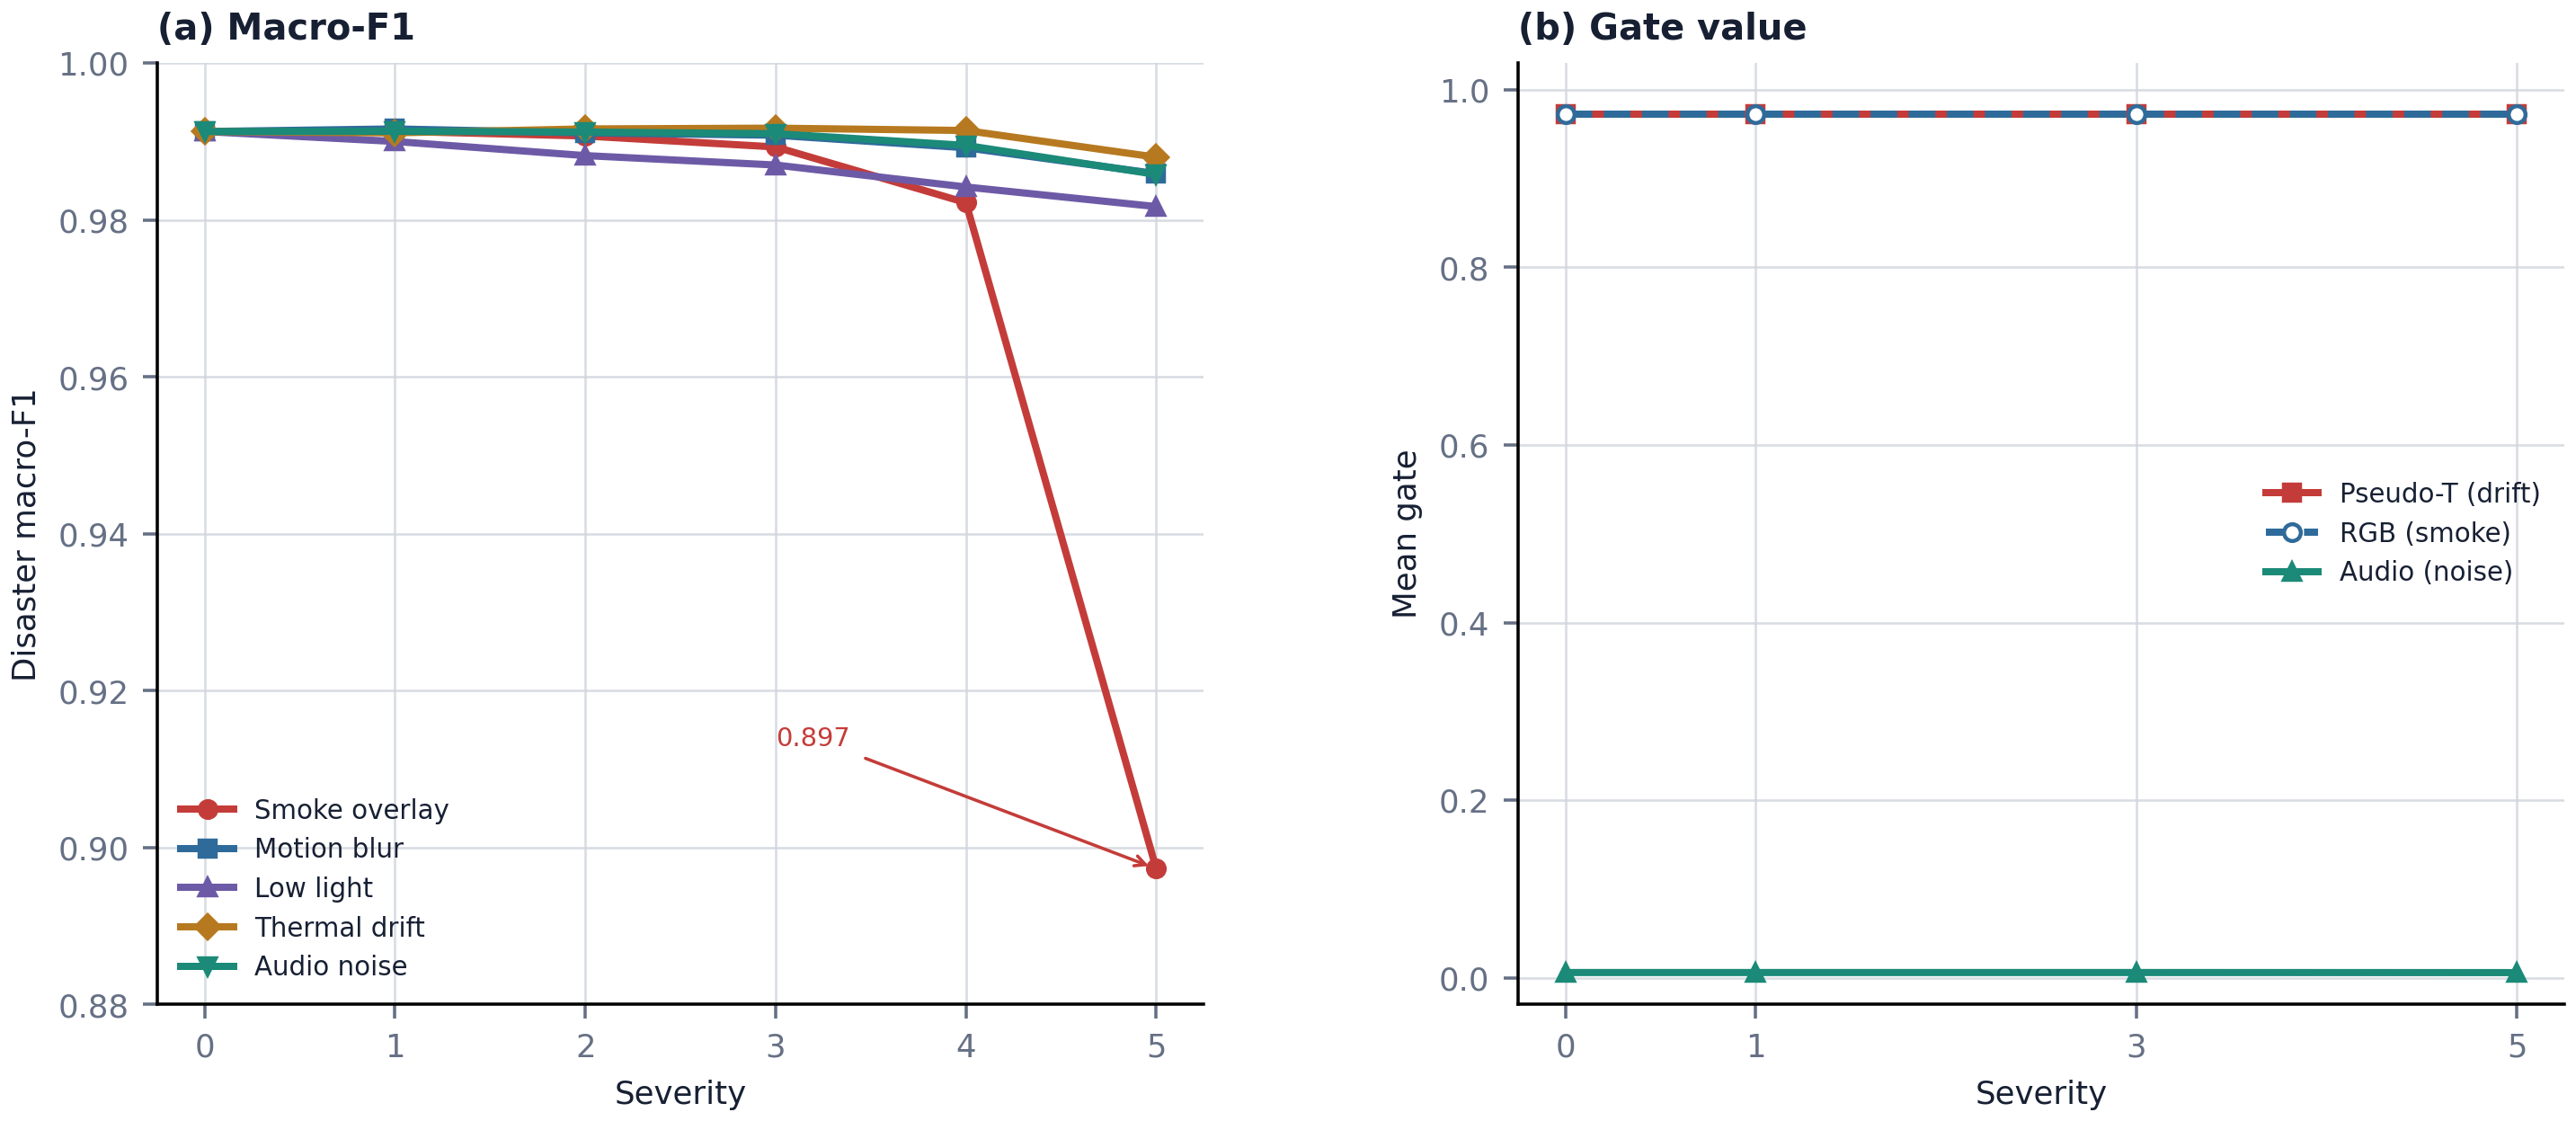
\includegraphics[width=\textwidth]{images/generated/fig_05_robustness.png}
\caption{Robustness evidence reconstructed from saved JSON logs. (A) AdapFuse-v1 disaster macro-F1 under five synthetic corruption sweeps; severe smoke reduces macro-F1 to 0.897. (B) The recorded gate associated with each corrupted input; the RGB (dashed) and pseudo-thermal curves coincide. RGB and pseudo-thermal gate means remain at 0.972 and the audio mean near 0.006 across severity; because these means include missing-modality rows (gate 0), the image gates stay saturated at $\approx$1.0 on every row with input. Hence robustness should be attributed to representation redundancy rather than demonstrated dynamic reweighting. The former hypothetical fixed-fusion trajectory has been removed.}
\label{fig:robustness_stress}
\end{figure}

Figure~\ref{fig:robustness_qualitative} grounds the aggregate sweep in one real FLAME test image processed under a clean input, a synthetic smoke overlay, and simulated RGB dropout. The predictions and gates are checkpoint outputs; the altered conditions themselves are synthetic.

\begin{figure}[H]
\centering
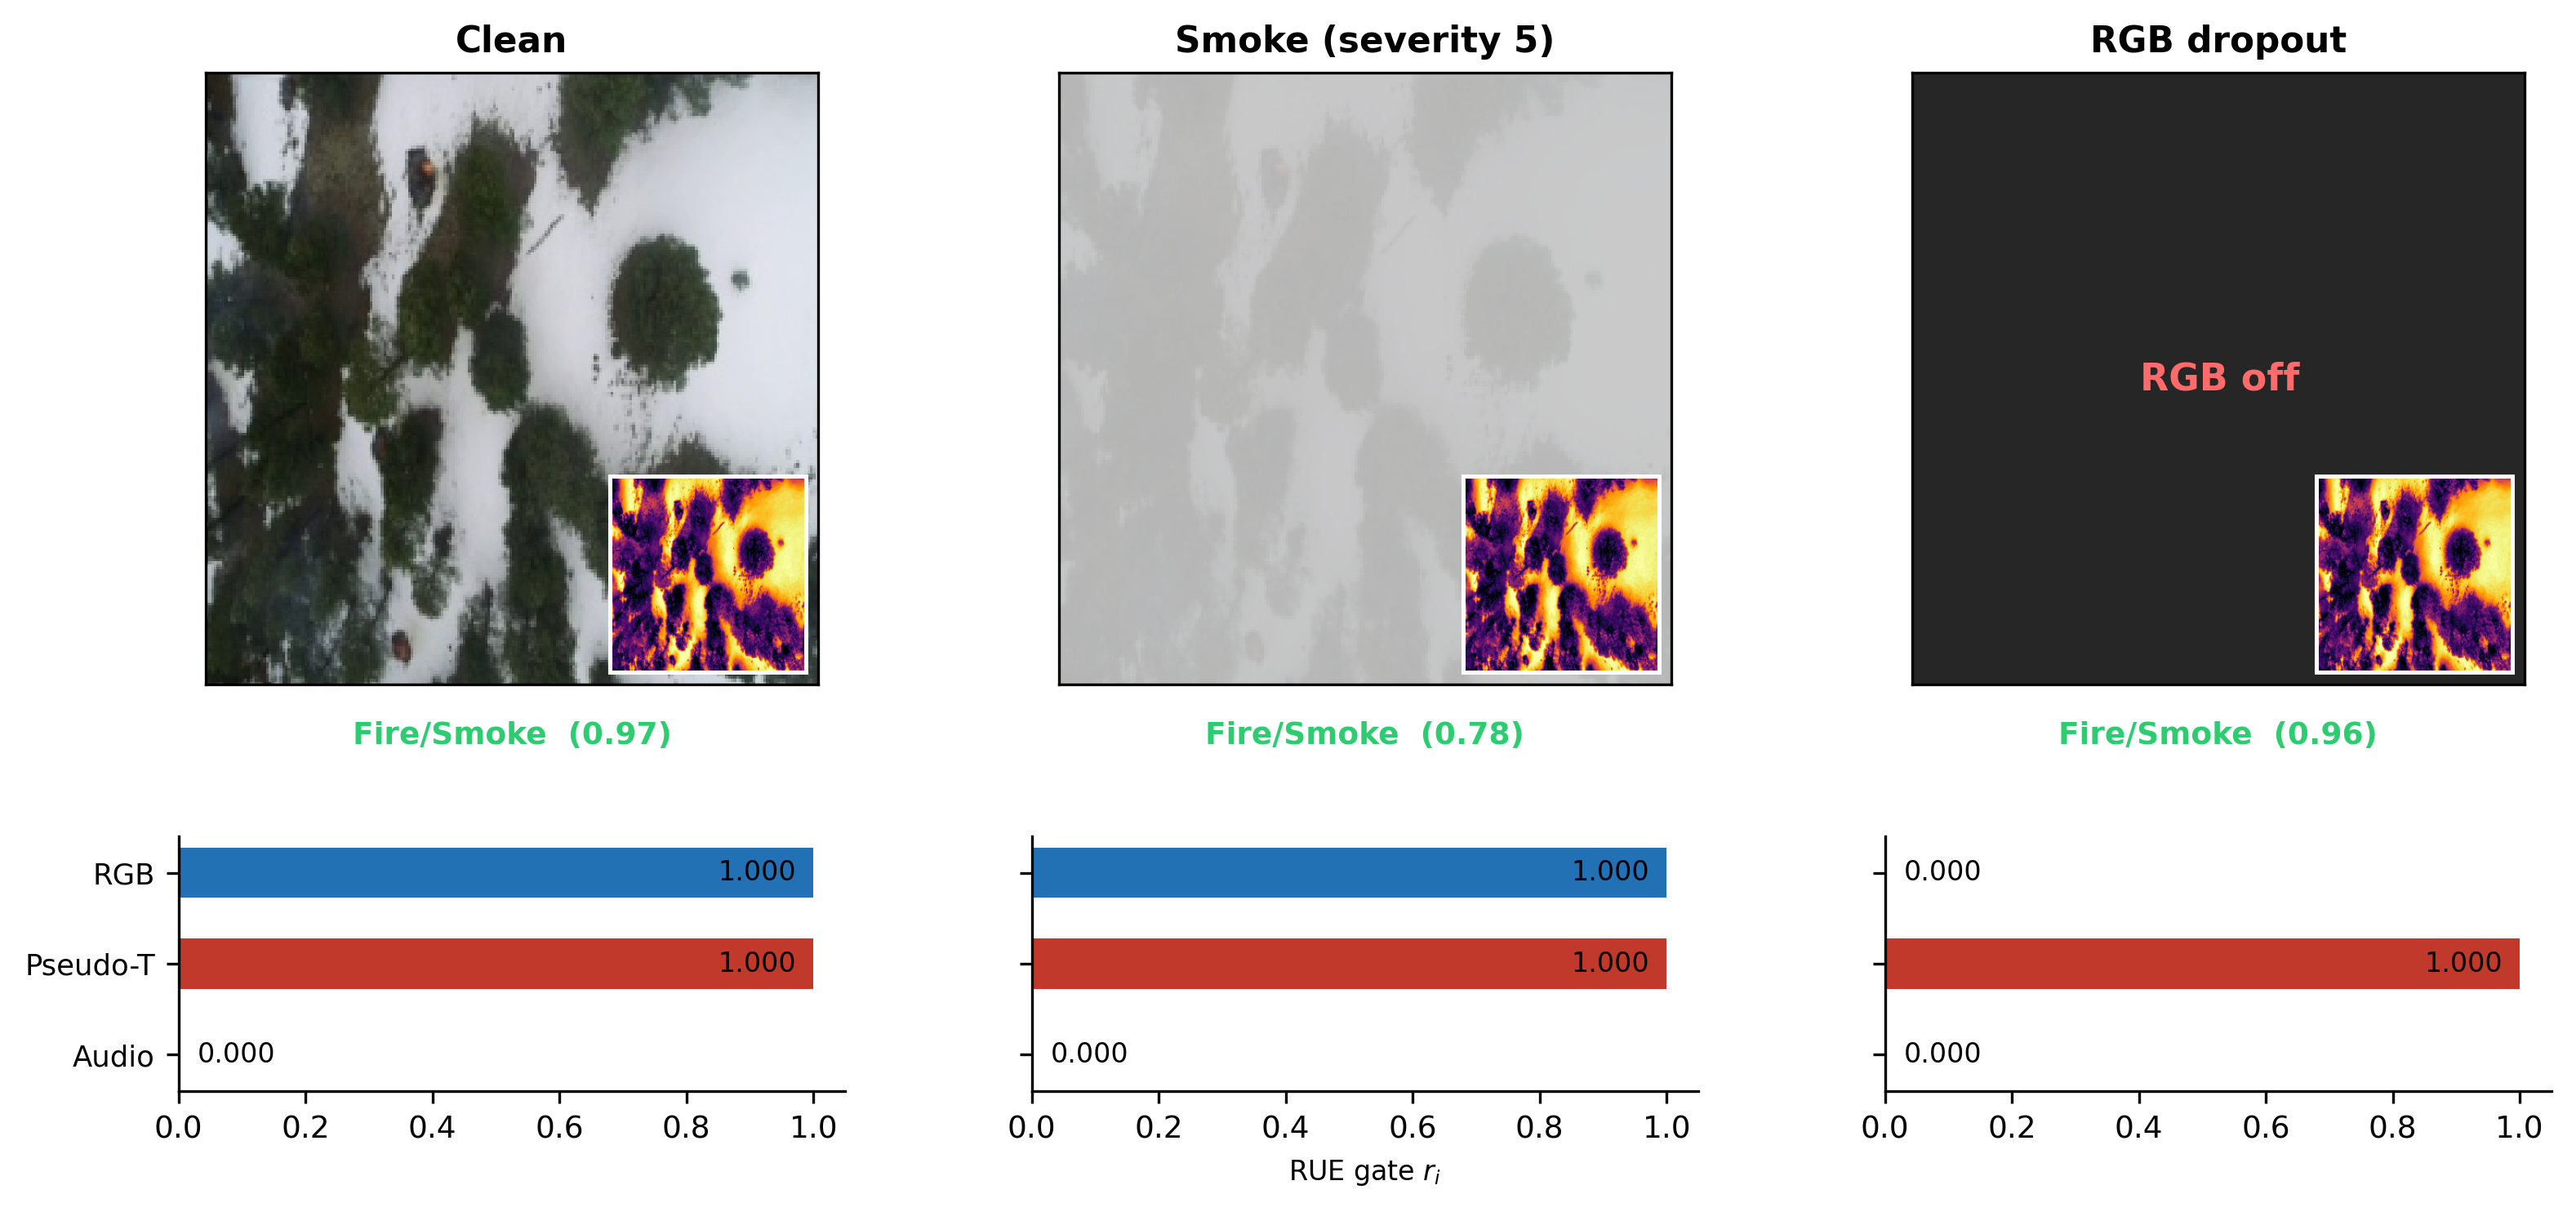
\includegraphics[width=\textwidth]{images/generated/fig_12_robustness_qualitative.png}
\caption{Checkpoint forward-pass outputs on one real FLAME RGB test frame (\texttt{flame\_012650}) under clean input, synthetic smoke overlay, and simulated RGB dropout. Text under each image gives the predicted class and confidence. The prediction is retained in this example. The inset is an RGB-derived pseudo-thermal map, not sensor IR. The RGB gate does not decline under smoke, so this example does not demonstrate corruption-sensitive reliability estimation.}
\label{fig:robustness_qualitative}
\end{figure}

\begin{enumerate}
    \item \textbf{Synthetic smoke overlay:} Disaster macro-F1 decreases from 0.9913 to 0.8973 at severity 5. Our mean RGB gate remains 0.9721 (the value obtained when every row with RGB has a gate of $\approx$1.0) rather than tracking the corruption; robustness is therefore more plausibly due to residual visual signal and redundancy with the RGB-derived pseudo-thermal input.
    \item \textbf{Pseudo-thermal drift:} Macro-F1 remains 0.9880 at severity 5, while the pseudo-thermal gate remains near 0.9721. This is a sensitivity result for transformed derived maps, not a radiometric sensor-drift experiment.
    \item \textbf{Motion blur:} Macro-F1 remains 0.9859 at severity 5, a 0.54\,pp decline from the clean 0.9913 baseline.
    \item \textbf{Low light:} Macro-F1 remains 0.9817 at severity 5, the second-largest decline after the smoke overlay.
    \item \textbf{Audio-noise transform:} Macro-F1 remains 0.9858 at severity 5. The audio gate is already near 0.006 before corruption and changes negligibly, consistent with the model largely ignoring this label-matched channel.
\end{enumerate}

\section{Component-Wise Ablation Study of the AdapFuse-v1 Architecture}
\label{sec:component_ablations}

Five single-component variants were trained on the same row-level split and evaluated on the held-out test set ($n=10{,}951$). Table~\ref{tab:ablation_results} reports their descriptive differences from our base run. Because the repository does not contain repeated seeds or confidence intervals, these comparisons indicate associations rather than causal component effects.

\begin{table}[H]
\centering
\caption{Component-wise AdapFuse-v1 variants on the row-level test split ($n=10{,}951$). Rows are separate saved training runs; no repeated seeds or confidence intervals are available.}
\label{tab:ablation_results}
\resizebox{\textwidth}{!}{%
\begin{tabular}{@{}llcccccc@{}}
\toprule
\textbf{Model Variant} & \textbf{Component Removed} & \textbf{Test Loss} & \textbf{Dis.\ F1} & \textbf{Vic.\ F1} & \textbf{Comb.\ F1} & \textbf{$\Delta$ Comb.\ F1} & \textbf{Loss Multiple} \\
\midrule
\textbf{AdapFuse-v1 (Base Teacher)} & \textbf{None (Full Architecture)} & \textbf{0.0020} & \textbf{0.9913} & \textbf{0.9836} & \textbf{0.9874} & \textbf{n/a} & \textbf{1.0$\times$} \\
\texttt{ablation\_no\_gru} & Single-step GRU Refinement & 0.0102 & 0.9863 & 0.9765 & 0.9814 & \textbf{$-$0.60 pp} & 5.1$\times$ \\
\texttt{ablation\_no\_attention} & Cross-Modal Attention & 0.0076 & 0.9894 & 0.9785 & 0.9839 & \textbf{$-$0.35 pp} & 3.8$\times$ \\
\texttt{ablation\_no\_quality\_tokens} & Quality Token Heads & 0.0108 & 0.9881 & 0.9800 & 0.9840 & \textbf{$-$0.34 pp} & 5.4$\times$ \\
\texttt{ablation\_no\_nuisance} & NuisanceAwareHead & 0.0092 & 0.9923 & 0.9821 & 0.9872 & \textbf{$-$0.02 pp} & 4.6$\times$ \\
\texttt{ablation\_no\_rue} & RUE Reliability Gating & 0.0094 & 0.9938 & 0.9812 & 0.9875 & $+$0.01 pp$^*$ & 4.7$\times$ \\
\bottomrule
\end{tabular}%
}
\footnotesize{$^*$The no-RUE run is 0.01 percentage points higher in combined F1 but has 4.7$\times$ the base run's loss. Our stress-test logs do not contain a matched no-RUE corruption baseline, and the learned gates are nearly constant, so robustness cannot be attributed to dynamic reliability tracking.}
\end{table}

\textbf{1. Single-Step GRU Refinement Changes the Learned Representation.}
Removing the GRU block (\texttt{ablation\_no\_gru}) corresponds to the largest difference in this suite: Combined F1 is 0.60 percentage points lower and victim-presence F1 is 0.71 points lower, while test loss is 5.1$\times$ higher. However, the implementation invokes the GRU with sequence length one (\texttt{fused.unsqueeze(1)}) and no carried-over hidden state, so each sample starts from a zero state and no information passes between frames. It therefore acts as a gated nonlinear refinement layer in these experiments; the result is not evidence of temporal smoothing, vibration invariance, or robustness across successive frames.

\textbf{2. Modality-Token Attention Outperforms Mean Pooling in This Run.}
Replacing the 4-head attention block with token mean pooling (\texttt{ablation\_no\_attention}) corresponds to 0.35 percentage points lower combined F1 and 0.51 points lower victim-presence F1, with a 3.8$\times$ higher loss. The attention operates over three globally pooled modality tokens, not localized spatial patches. Moreover, the pseudo-thermal token is derived from the RGB image, so this experiment supports learned modality-level interaction but not independent RGB--thermal spatial correspondence.

\textbf{3. Learned Quality Features Are Associated with Lower Test Loss.}
Removing the dedicated 16-dimensional quality heads (\texttt{ablation\_no\_quality\_tokens}) corresponds to a 0.34-point lower combined F1 and a test loss of 0.0108 (5.4$\times$ the base run). This shows that the learned quality features are useful within the fitted architecture, but it does not establish calibrated uncertainty or detection of physical sensor degradation because no degradation targets are supplied during training.

\textbf{4. The Nuisance Variant Does Not Establish Nuisance Supervision.}
The no-nuisance run has a 4.6$\times$ higher loss but nearly unchanged combined F1. In our trainer, \texttt{nuisance\_gt=None}, so the base model's nuisance loss is also zero. The difference between these saved runs cannot therefore be interpreted as evidence that an auxiliary nuisance objective regularizes false-alarm features; repeated controlled runs with nuisance labels are required.

\section{Backbone Exploration and Architectural Augmentations}
\label{sec:backbone_variants}

\subsection{High-Capacity Visual Scaling: EfficientNet-B0 and MobileViT-XXS}
\begin{itemize}
    \item \textbf{EfficientNet-B0 (RGB):} Replacing MobileNetV3-Small with EfficientNet-B0~\cite{tan2019efficientnet} achieved the highest score among our runs: \textbf{99.24\% Combined F1} (Disaster F1: 99.23\%, Victim-presence F1: \textbf{99.24\%}, Victim-presence Accuracy: \textbf{99.47\%}). These are scene-level labels; no person size or location is evaluated.
    \item \textbf{MobileViT-XXS Hybrid Transformer:} Incorporating MobileViT-XXS~\cite{mehta2022mobilevit} for the RGB stream achieved \textbf{98.99\% Combined F1} and \textbf{99.16\% Victim-presence F1}. This supports the backbone as a competitive scene classifier on the present split, but does not by itself demonstrate survivor localization or edge-device operation.
    \item \textbf{EfficientNet-B0 (Pseudo-thermal):} Applying EfficientNet-B0 to the 1-channel RGB-derived maps achieved \textbf{98.80\% Combined F1} and \textbf{99.50\% Disaster Accuracy}. Because these inputs are algorithmically derived rather than radiometric LWIR measurements, the result does not test separation of physical heat sources from solar-heated clutter.
\end{itemize}
The RGB-only and pseudo-thermal-only versions of these backbones are reported in Tables~\ref{tab:unimodal_rgb} and~\ref{tab:unimodal_thermal}; with the backbone held fixed, the fused models score between 0.00 and 0.36 combined-F1 points higher.

\subsection{Acoustic Backbone Variants: GDBlock vs.\ Pretrained PANNS}
Experiments comparing acoustic encoders (Table~\ref{tab:main_results}, Ranks 10, 16, 20) show that the multi-scale dilated \textbf{GDBlock} architecture reaches \textbf{98.63\% Combined F1} (0.0036 loss), while \textbf{PANNS-CNN6}~\cite{kong2020panns} reaches \textbf{98.25\%} (0.0038 loss). Because ESC-50 clips are reused and label-matched rather than synchronized to the visual scene, these results are most directly evidence of an alignment bottleneck; they are not an experiment with measured UAV rotor noise. With the audio gate near zero, the 0.38-point gap between the two backbones mostly reflects how the rest of the network trains alongside each encoder, not the quality of disaster-relevant acoustic features, and neither result demonstrates audio--visual fusion. Trained alone (Table~\ref{tab:unimodal_audio}), both encoders reach the same degenerate solution, which confirms that their fused scores come from the visual streams.

\subsection{Two-Sensor Subset Deployments}
\label{sec:two_sensor}
Evaluating two-channel subsets shows that \textbf{RGB + pseudo-thermal} reaches \textbf{98.50\% Combined F1} and \textbf{pseudo-thermal + audio} reaches \textbf{98.05\%}. These are metadata-channel ablations rather than hardware payload experiments. In particular, pseudo-thermal is computed from visible RGB, so the latter result does not establish a fallback for zero-visibility night or heavy-smoke operation: when the RGB frame is dark or occluded, the pseudo-thermal map derived from it is degraded in the same way. Likewise, the RGB + pseudo-thermal result combines two views of the same sensor and does not test fusion of independent sensors. A fallback evaluation requires independent LWIR hardware.

\subsection{Spatial Attention and Domain Prompt Tokens}
The \textbf{Spatial Attention} augmentation (\texttt{adaptfuse\_v1\_spatial\_attn}, 98.44\% F1) and \textbf{Domain Prompt Tokens} (\texttt{adaptfuse\_v1\_domain\_prompts}, 98.49\% F1) show that both modules can be added to the architecture with little change in row-level performance ($-0.30$ and $-0.25$ combined-F1 points relative to the 98.74\% base). Both are evaluated on the same row-level split as the base model, and the domain prompts are not supervised with condition labels; these results therefore show only that the modules do not degrade within-collection performance, not that they improve behaviour in specific flight regimes. Testing that claim would require held-out data from different altitudes, illumination, weather or sensor payloads.

\section{Error Analysis}
\label{sec:failure_gallery}

The near-ceiling aggregate metrics reported in Table~\ref{tab:main_results} can obscure specific failure modes. Figure~\ref{fig:failure_gallery} surfaces genuine misclassifications discovered by re-running trained checkpoints across the natural test set.

\begin{figure}[H]
\centering
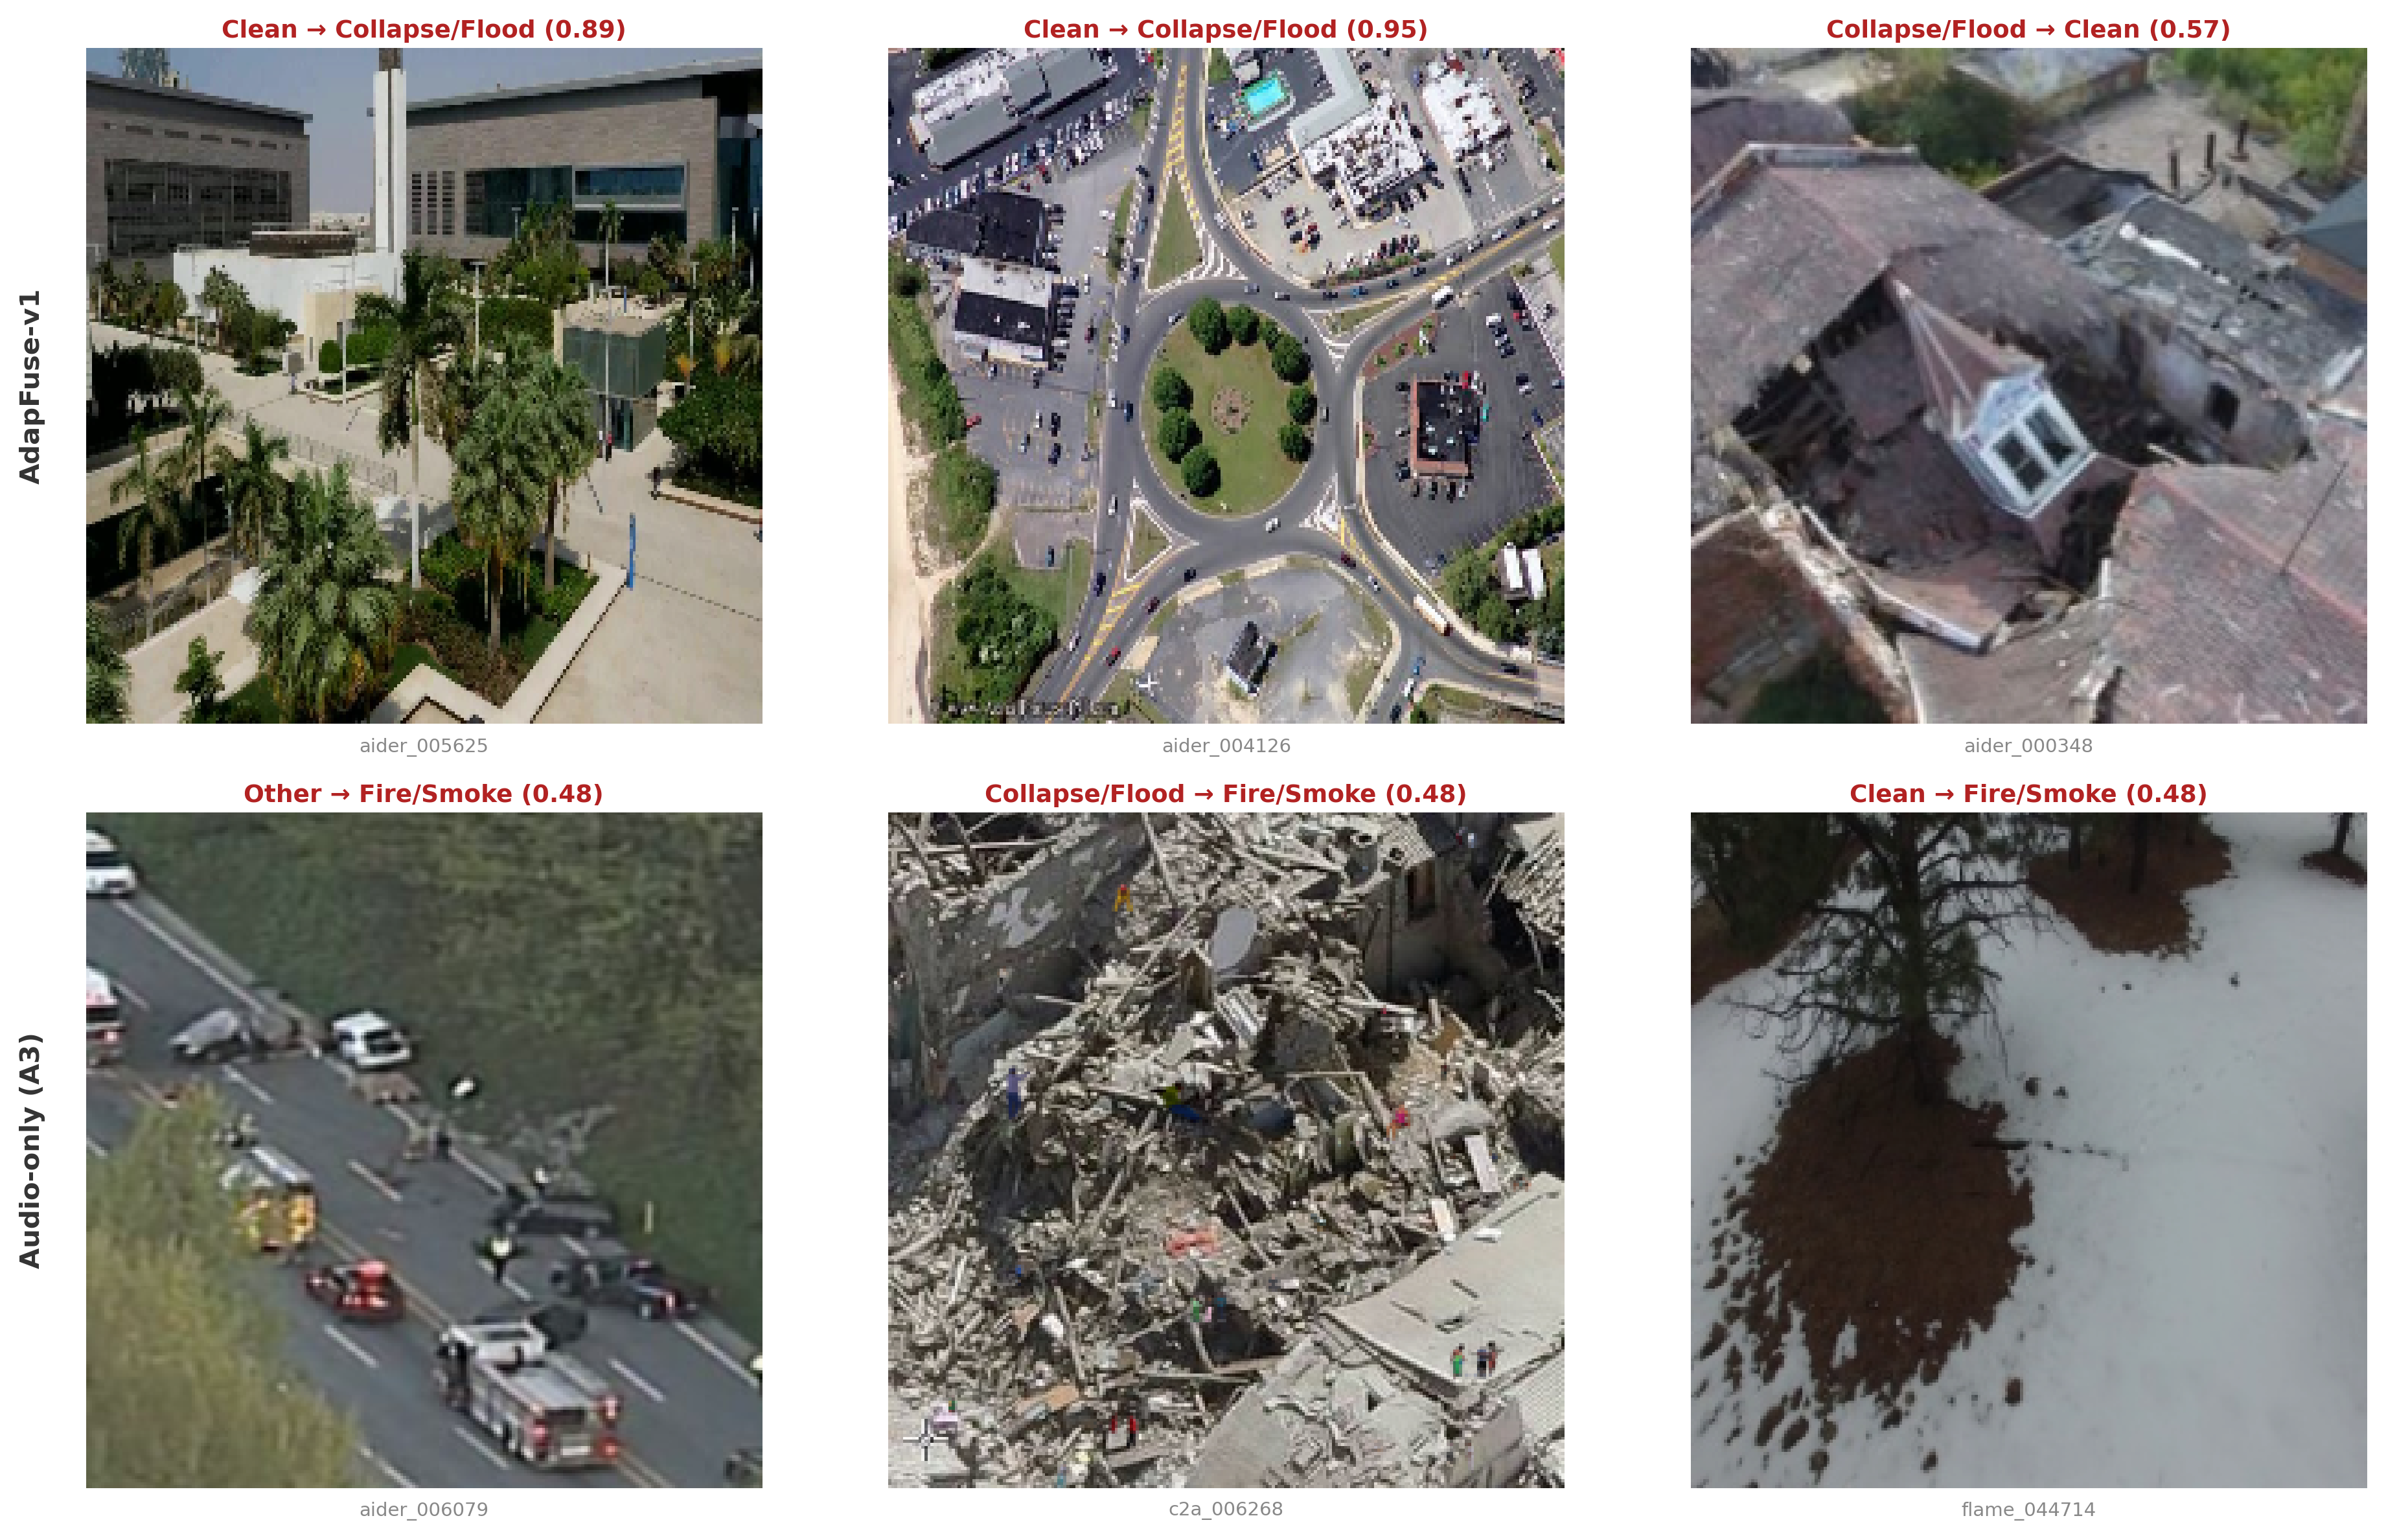
\includegraphics[width=\textwidth]{images/generated/fig_13_failure_gallery.png}
\caption{Real misclassifications from re-running trained checkpoints on the natural-distribution test set. Panel titles give true $\rightarrow$ predicted class (confidence). Top row: AdapFuse-v1 errors are rare (8 found across 1{,}280 sampled test rows, consistent with its 99.44\% disaster accuracy) and concentrate on visually ambiguous clean-vs-collapse scenes (e.g.\ dense urban/structural clutter mistaken for collapse debris). Bottom row: the audio-only baseline (A3, 38.2\% disaster F1) fails much more frequently (121 errors in a smaller sample), consistently defaulting to a Fire/Smoke prediction regardless of true class, which is direct visual evidence for the audio-signal-quality bottleneck discussed throughout this chapter.}
\label{fig:failure_gallery}
\end{figure}

\section{Summary of Key Findings}

\begin{enumerate}
    \item \textbf{Dense Object Detection Benchmark:} High-capacity YOLO26s (CLAHE) achieves $77.10\%\, \text{mAP}_{50}$ on D-Fire, while RT-DETRv2-R18 reaches $73.80\%$ and YOLO11n attains $72.25\%$.
    \item \textbf{HPG Efficiency--Accuracy Trade-off:} Hazard-YOLO26n reaches $70.53\%\, \text{mAP}_{50}$ in $1.96\,\text{hours}$ versus $71.47\%$ in 4.45 hours for baseline YOLO26n. The shorter saved run is useful evidence of lower training cost, but not a controlled proof of faster convergence.
    \item \textbf{Multi-Task Prototype:} Curriculum warmup and stop-gradient isolation recover scene classification to $99.26\%$ disaster accuracy and $98.57\%$ combined F1. The same saved evaluation reports detection $\text{mAP}_{50}=0.0$, so successful joint localization is not established.
    \item \textbf{Fusion versus RGB-only:} On the row-level split, AdapFuse-v1 (98.74\% combined F1) does not exceed the RGB-only baseline (98.85\%), and the no-RUE variant (98.75\%) matches it; the fused inputs are RGB-derived or label-matched, so no fusion accuracy gain is shown.
    \item \textbf{Unimodal Backbones:} With three backbones per modality, the best RGB-only model (MobileViT-XXS, 98.99\%) matches the best-but-one fused model, and the best pseudo-thermal-only model (EfficientNet-B0, 98.60\%) improves on ResNet-18 by 1.17 points. With the backbone held fixed, fusion adds 0.00--0.36 points. PANNS-CNN6 and GDBlock audio-only runs collapse to identical degenerate predictions.
    \item \textbf{Public Benchmarks:} Under the published AIDER 4:1:2 protocol, RGB-only EfficientNet-B0 reaches 94.00\% macro-F1 against 88.5\% for WATT-EffNet (trained from scratch). Under the official cross-camera FLAME protocol it reaches 83.72\% accuracy against 76.23\% for Xception, while in-domain validation F1 is 99.9\% for every model. AdapFuse-v1 is below RGB-only EfficientNet-B0 on both.
    \item \textbf{Component Variants:} The base run outperforms the no-GRU, no-attention, and no-quality-feature runs by 0.60, 0.35, and 0.34 F1 points, respectively. These single-run differences are descriptive; the GRU receives one step, reliability has no degradation targets, and the nuisance loss is zero.
    \item \textbf{Scene-Level Backbone Results:} EfficientNet-B0 reaches $99.24\%$ Combined F1 and MobileViT-XXS reaches $98.99\%$ on the row-level split. These results concern victim presence, not person localization.
    \item \textbf{Row-Level Error and Workstation Speed:} AdapFuse-v1 reports 0.73\% row-level scene-classification FPR, ECE 0.0337, and 14.26\,ms inference on an RTX 5090 workstation (32\,GB VRAM). Neither operational false-alarm reduction nor embedded-UAV speed has been validated.
    \item \textbf{Split and Source Effects:} Under a capture-group-aware split, combined macro-F1 falls from 98.74\% to 89.14\% (single seed). Victim presence is fully determined by source dataset in the grouped test set, so aggregate scores cannot separate person or hazard recognition from dataset recognition.
    \item \textbf{Reliability Gates:} In the row-level model the RGB and pseudo-thermal gates are saturated at $\approx$1.0 and the audio gate at $\approx$0.011 on rows with each input, unchanged under every synthetic corruption; the grouped retraining instead saturates the audio gate at 1.0 and switches pseudo-thermal off on 43.5\% of rows. The gates act as run-dependent on/off switches, and the RUE is not shown to track degradation.
\end{enumerate}
